%DIF PREAMBLE EXTENSION ADDED BY LATEXDIFF
%DIF UNDERLINE PREAMBLE %DIF PREAMBLE
\RequirePackage[normalem]{ulem} %DIF PREAMBLE
\RequirePackage{color}\definecolor{RED}{rgb}{1,0,0}\definecolor{BLUE}{rgb}{0,0,1} %DIF PREAMBLE
\providecommand{\DIFadd}[1]{{\protect\color{blue}\uwave{#1}}} %DIF PREAMBLE
\providecommand{\DIFdel}[1]{{\protect\color{red}\sout{#1}}}                      %DIF PREAMBLE
%DIF SAFE PREAMBLE %DIF PREAMBLE
\providecommand{\DIFaddbegin}{} %DIF PREAMBLE
\providecommand{\DIFaddend}{} %DIF PREAMBLE
\providecommand{\DIFdelbegin}{} %DIF PREAMBLE
\providecommand{\DIFdelend}{} %DIF PREAMBLE
%DIF FLOATSAFE PREAMBLE %DIF PREAMBLE
\providecommand{\DIFaddFL}[1]{\DIFadd{#1}} %DIF PREAMBLE
\providecommand{\DIFdelFL}[1]{\DIFdel{#1}} %DIF PREAMBLE
\providecommand{\DIFaddbeginFL}{} %DIF PREAMBLE
\providecommand{\DIFaddendFL}{} %DIF PREAMBLE
\providecommand{\DIFdelbeginFL}{} %DIF PREAMBLE
\providecommand{\DIFdelendFL}{} %DIF PREAMBLE
%DIF END PREAMBLE EXTENSION ADDED BY LATEXDIFF

%\documentclass[11pt]{sigplanconf}
%\nocaptionrule

% \documentclass[twocolumn,9pt]{article}
% \documentclass[twocolumn,10pt]{acm_proc_article-sp}

% \documentclass{acm_proc_article-sp}

\documentclass[10pt]{sigplanconf}

\date{} % \vspace*{-0.2in}}

% Make sure to put back 

\newcommand{\punt}[1]{}
\newcommand{\CC}[1]{{\large \textbf{\color{red}CC:} \emph{#1} \newline}}
\newcommand{\unedited}[1]{\noindent \textbf{\color{red}\texttt{<unedited>}} \indent \emph{#1} \newline \textbf{\color{red}\texttt{</unedited>}} \newline}

\usepackage{soul}
\usepackage{endnotes,xspace}

\newcommand{\footnotenonumber}[1]{{\def\thempfn{}\footnotetext{\small #1}}}
\usepackage[normalem]{ulem}
\usepackage{graphicx}

\usepackage{mathptmx} % rm & math
\usepackage[scaled=0.90]{helvet} % ss
\usepackage{courier} % tt
% \normalfont
\usepackage[T1]{fontenc}
\usepackage{algorithm}
\usepackage{algorithmic}
\usepackage{tgtermes}
\usepackage{amsmath,amssymb}
% \usepackage{lmodern}
% \usepackage{times}
\usepackage{subfigure}
\usepackage{url}
\urlstyle{rm}
\usepackage[
      colorlinks=false,    %no frame around URL
      urlcolor=black,    %no colors
      menucolor=black,    %no colors
      linkcolor=black,    %no colors
]{hyperref}

\usepackage{color}
\usepackage{listings}
\usepackage{amsmath}
\usepackage{amsfonts}
\usepackage{amssymb}
\usepackage{comment} 
\usepackage{setspace}
\singlespacing
%\onehalfspacing
\newtheorem{thm}{Theorem}
\newtheorem{prop}[thm]{Proposition}
\newtheorem{cor}[thm]{Corollary}
\newtheorem{lem}[thm]{Lemma}
\newtheorem{defn}[thm]{Definition}

\newcommand{\cfunction}[1]{{\bf \tt #1}}
\newcommand{\malloc}{\cfunction{malloc}}
\newcommand{\realloc}{\cfunction{realloc}}
\newcommand{\free}{\cfunction{free}}
\newcommand{\madvise}{\cfunction{madvise}}
\newcommand{\brk}{\cfunction{brk}}
\newcommand{\sbrk}{\cfunction{sbrk}}
\newcommand{\mmap}{\cfunction{mmap}}
\newcommand{\munmap}{\cfunction{munmap}}
\newcommand{\mprotect}{\cfunction{mprotect}}
\newcommand{\mlock}{\cfunction{mlock}}
\newcommand{\fixme}[1]{{\color{red}[\textsf{#1}]}}


\hyphenation{app-li-ca-tion}
\hyphenation{Die-Hard}
\hyphenation{Ar-chi-pe-la-go}
\hyphenation{buf-fer}
\hyphenation{D-threads}
\hyphenation{Heap-Layers}
\hyphenation{wait-Token}
\hyphenation{mul-ti-threa-ded}
\hyphenation{me-m-ory}

\hyphenation{pthread-create}
\hyphenation{pthread-self}
\hyphenation{pthread-mutex-lock}
\hyphenation{pthread-mutex-unlock}

\newcommand{\cheetah}{{\scshape Cheetah}}
\newcommand{\Cheetah}{{\scshape Cheetah}}
\newcommand{\Predator}{{\scshape Predator}}
\newcommand{\Sheriff}{{\scshape Sheriff}}
\newcommand{\sheriff}{{\scshape Sheriff}}
\newcommand{\Grace}{{\scshape Grace}}
\newcommand{\grace}{{\scshape Grace}}
\newcommand{\SheriffProtect}{\textsc{Sheriff-Protect}}
\newcommand{\sheriffProtect}{\textsc{Sheriff-Protect}}
\newcommand{\sheriffprotect}{\textsc{Sheriff-Protect}}
\newcommand{\SheriffDetect}{\textsc{Sheriff-Detect}}
\newcommand{\sheriffDetect}{\textsc{Sheriff-Detect}}
\newcommand{\sheriffdetect}{\textsc{Sheriff-Detect}}
\newcommand{\pthreads}{\texttt{pthreads}}
\newcommand{\eat}[1]{}
\newcommand{\todo}[1]{{\color{red}[\textsf{#1}]}}


\definecolor{lightgray}{rgb}{.9,.9,.9}
\definecolor{darkgray}{rgb}{.4,.4,.4}
\definecolor{purple}{rgb}{0.65, 0.12, 0.82}

\lstdefinelanguage{c++threads}[]{c++}{
  morekeywords={pthread_create,pthread_join},
  keywordstyle=\color{blue}\bfseries,
  ndkeywords={class, export, boolean, throw, implements, import, this},
  ndkeywordstyle=\color{darkgray}\bfseries,
  identifierstyle=\color{black},
  sensitive=false,
  comment=[l]{//},
  morecomment=[s]{/*}{*/},
  commentstyle=\color{purple}\ttfamily,
  stringstyle=\color{red}\ttfamily,
  morestring=[b]',
  morestring=[b]"
}
\lstset{
   language=c++threads,
   backgroundcolor=\color{lightgray},
   extendedchars=true,
   basicstyle=\footnotesize\ttfamily,
   showstringspaces=false,
   showspaces=false,
   numbers=none,
   numberstyle=\footnotesize,
   numbersep=9pt,
   tabsize=2,
   breaklines=true,
   showtabs=false,
   captionpos=b
}
%\lstset{language=c++threads, basicstyle=\ttfamily\scriptsize,frame=trbl,tabsize=4} % ,numbers=left,numberstyle=\tiny}

\definecolor{Gray}{cmyk}{0,0,0,0.5}

\begin{document}
\special{papersize=8.5in,11in}
\setlength{\pdfpageheight}{\paperheight}
\setlength{\pdfpagewidth}{\paperwidth}

\conferenceinfo{CGO 2016}{Month d--d, 20yy, City, ST, Country} 
\copyrightyear{2016} 
\copyrightdata{978-1-nnnn-nnnn-n/yy/mm} 
\doi{nnnnnnn.nnnnnnn}

%\CopyrightYear{2015}
%\copyrightdata{XXX-X-XXXXX-XXX-X/XX/XX}

\title{{\huge \bf \Cheetah{}}: Detecting False Sharing \\ Efficiently and Effectively}

%\begin{comment}
\authorinfo{Double blind review}{}{}

%\authorinfo{Tongping~Liu \and Emery~D.~Berger}
%{School of Computer Science \\
%University of Massachusetts Amherst \\
%Amherst, MA 01003 \\
%{\{tonyliu,emery\}@cs.umass.edu}
%}
%\end{comment}

\maketitle

\begin{abstract}
%False sharing occurs when multiple threads, running on different cores with separate caches, access logically independent words in the same cache line. 

%Multicore processors are ubiquitous across the full computing spectrum, from phones, desktops, to high-end servers. 
False sharing is a notorious performance problem that may occur in multithreaded programs running on ubiquitous multicore hardware. It can dramatically degrade the performance by up to an order of magnitude, significantly hurting the scalability. Identifying false sharing is challenging. Existing tools either introduce significant performance overhead that can block their uses in deployed software or cannot provide adequate information to guide optimization.
%On the one hand, it is necessary to monitor memory accesses in order to report problematic instructions and data objects, 
%accurately and distinguish them with true sharing, but that usually incurs very high performance overhead. On the other hand, existing lightweight techniques have limited precisions in detecting false sharing and often provide inadequate information to guide optimization.
%that can dramatically degrade the performance of multithreading programs by up to an order of magnitude. 
%The hardware trend, including adding more cores into the same machine, introducing the Non-Uniform-Memory-Access (NUMA) architecture, or increasing the size of a cache line, will further degrade the performance of false sharing problems, making the task of detecting more urgent. 
%Existing detection tools have different types of shortcomings: most tools cannot report precise information about false sharing; some may introduce too much performance overhead; some have a lot of limitations on applications or the environment; all tools cannot assess how much performance improvement by fixing a specific false sharing problem. 

\sloppy
We present \cheetah{} in this paper, a profiler that detects false sharing both {\bf efficiently} and {\bf effectively}. \cheetah{} leverages lightweight hardware performance monitoring units that are available on most existing modern hardware to sample memory accesses. \cheetah{} is the first tool that can quantify the optimization potential of a problem without actual fixes, by utilizing the latency information of every sampled access. \cheetah{} precisely reports false sharing and provides insightful optimization guidance for programers, with adding less than $7\%$ runtime overhead. \Cheetah{} is ready for real deployment. 

%Unlike prior work, \cheetah{} quantitatively assesses the potential gains of fixing each false sharing instance, so programmers can focus on the most severe problems only. %\cheetah{} provides the most comprehensive information that can assist users to fix false sharing problems. 
%We evaluate \cheetah{} on two benchmark suites (Phoenix and PARSEC), and multiple real applications. 
%According to our evaluation, \Cheetah{} can detect false sharing, . 
%Guided by \Cheetah{}, we obtain significant performance improvement. %ready to be used in deployment environment because of its negligible performance overhead (3\%) and its effectiveness.  

\keywords{Multithreading, False Sharing, Memory Access Sampling, Lightweight Profiling}

\end{abstract}

%  Language-based approaches require programmers to write their code in specialized languages. 


\punt{
\category{D.1.3}{Programming Techniques}{Concurrent Programming--Parallel Programming}
\category{D.2.5}{Software Engineering}{Testing and Debugging--Debugging Aids}

\terms
Design, Reliability, Performance

\keywords
False Sharing, Detection Tools, Performance 
}


%%%%%%%%%%%%%%%%%%%%%%%%%%%%%%%%%%%%%%%%%%%%%%%%%%%%%%%%%%%%%%%%%%%%%%%%%%%%%%%%%%%%%%%%%%%%%
%%%%%%%%%%%%%%%%%%%%%%%%%%%%%%%%%%%%%%%%%%%%%%%%%%%%%%%%%%%%%%%%%%%%%%%%%%%%%%%%%%%%%%%%%%%%%

\section{Introduction}
\begin{comment}
Multicore architectures 
cache system
sharing and false sharing
existing tools for false sharing
limitations
contributions
structures
\end{comment}

Modern computer systems, such as server nodes, desktops, and smart phones, employ multiple cores to explore high parallelism. To bridge the speed gap between CPU and main memory, multi-level cache hierarchies are used to block data for fast accesses. Typically in the memory hierarchy, there are private layers associated with each core and shared layers between cores. For example, Intel Sandy Bridge processors have private L1 and L2 caches, as well as shared L3 caches. Moreover, IBM POWER8 processors have L1, L2 private caches, and L3, L4 shared caches.
To facilitate programming and guarantee the correctness, there are complex cache coherency protocols~\cite{MESI} implemented in the hierarchy.

The complex memory hierarchies in multi-core systems may suffer from various performance issues, such as poor data locality~\cite{ibs-sc,ibs-ispass}, intensive cache contention~\cite{ibs-sc2}, and bandwidth underutilization~\cite{Dramon}. Among them, false sharing is a common programming flaw that can significant hurt a parallel program's performance and scalability. False sharing occurs between threads, when these threads (1) run on cores with private caches, (2) access different words of a cache line, unlike true sharing between threads, which access the same word, and (3) at least one access is a write. Given the cache coherence protocol, threads with writing the words keep invalidating the cache line in all private caches and flushing the data to the shared caches. Thus, when some threads use the data, they need to load the data from the shared cache, rather than the fast private one.

%Multicore processors are ubiquitous, from phones, desktops, to high-end servers.
%False sharing occurs when multiple tasks, running on different cores with private L1 caches, access logically independent words in the same cache line. When a thread modifies data of a cache line, the underlying cache coherence protocol (inside hardware) silently invalidates the duplicates of this cache line on other cores. Unnecessary synchronizations caused by false sharing can dramatically degrade the performance of parallel software by up to an order of magnitude ~\cite{falseshare:effect}. A simple example shown in Figure~\ref{fig:penalty} also exemplifies this catastrophic performance effect of false sharing. Figure~\ref{} shows how false sharing occurs in a typical multi-core platform.


%The hardware trend, including adding more cores into the same machine, introducing the Non-Uniform-Memory-Access (NUMA) architecture, or increasing the size of a cache line, will further degrade the performance of false sharing problems, making the task of detecting even more urgent. 

\begin{figure*}[htbp]
\centering
\subfigure[Parallel Programs]{%
   \label{fig:penaltycode}
   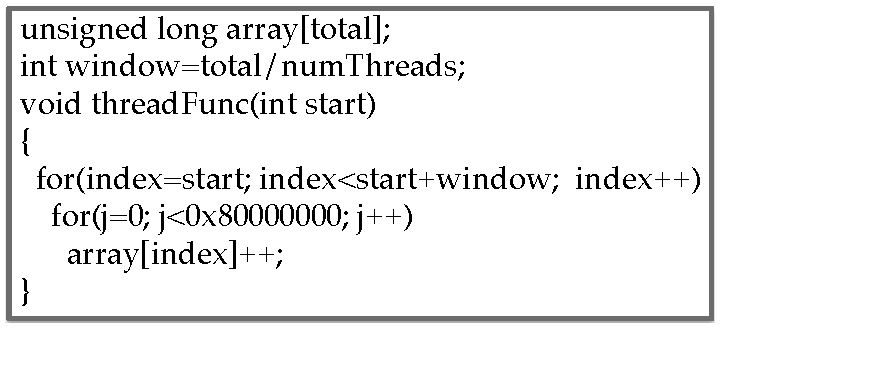
\includegraphics[width=2.8in]{figure/fscode}

}%
\hspace{30pt}
\subfigure[Performance Degradation]{%
   \label{fig:penaltyfig}
   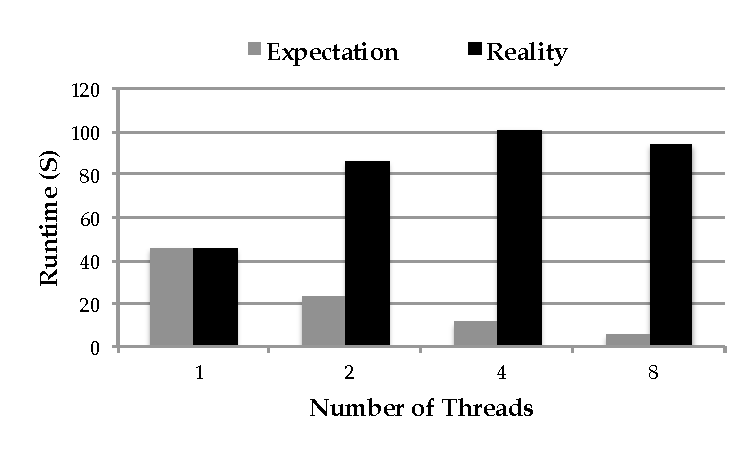
\includegraphics[width=2.4in]{figure/penalty}
}
\caption{
A false sharing example inside a multithreaded program (a) causes $13\times$ performance degradation (b) on a 8-core machine.
\label{fig:penalty}}
\end{figure*}

% Now we will talk about existing tools. 
As a concrete example, as shown in Figure~\ref{fig:penalty}, careless code design can lead to false sharing: multiple threads access adjacent elements of {\tt array} that reside in the same cache line. When parallelize this loop with threads, one can see from Figure~\ref{fig:penaltyfig} that the scalability (in red) is much worse than expected (in green). Therefore, it is important to eliminate false sharing to obtain high performance and scalability. 
Unlike true sharing, false sharing is avoidable. As threads unnecessarily share the same cache line, we can pad the data to force each thread access a different cache line. Although the solution for false sharing is straightforward, detecting it is difficult and even impossible with manual effort only, especially for a code with hundreds of thousands of lines. Thus, there is a demand for tool to pinpoint false sharing and provide insightful optimization guidance.

However, existing generic performance tools do not provide details about false sharing. For example, well-known profilers such as gprof~\cite{gprof}, HPCToolkit~\cite{ibs-sc}, TAU~\cite{Malony-etal:2008:TAU}, and VTune~\cite{Intel:VTune} report time consumption and cache miss counts, but do not point that whether the long running time and large amount of cache misses are caused by false sharing or not. On the other hand, existing specific tools targeting false sharing detection also lack in several ways. First, some tools~\cite{falseshare:binaryinstrumentation1,detect:ptu,detect:intel,falseshare:binaryinstrumentation2,DProf, qinzhao, OSdetection, mldetect, Wicaksono11detectingfalse, openmp} do not distinguish true and false sharing, requiring manual efforts to identify optimization opportunities. Second, some tools~\cite{falseshare:binaryinstrumentation1,falseshare:binaryinstrumentation2,falseshare:simulator, Predator} introduce high runtime overhead, preventing them from practical usage. Third, some tools require special features from OS~\cite{OSdetection}, compilers~\cite{Predator}, and applications~\cite{sheriff}. Fourth, to the best of our knowledge, no prior tool assesses the benefit from eliminating the false sharing. Without this information, many optimization efforts may lead to trivial performance improvement.

\vspace{0.2in}

To address these issues, we develop \cheetah{} with the following three contributions:
\begin{itemize} 
\item \cheetah{} can report precise information about false sharing problems. Like those precise tools, e.g. Sheriff~\cite{sheriff} and Predator~\cite{Predator}, it will pinpoint the lines of code where those variables or objects have false sharing problems. More than that, \cheetah{} can further pinpoint statements exercising false sharing problems, which can help programmers fix found problems. 

\sloppy
\item Based on hardware performance monitoring units (PMU), \cheetah{} significantly reduces the runtime overhead of detection, with only 5\% average performance overhead and 10\% maximum overhead. The performance overhead is similar to recent work~\cite{mldetect, openmp}, but with more precise information and more effectiveness.
  
\item Unlike all existing tools, \Cheetah{} can quantify the performance impact of false sharing instances based on the memory access latency information provided by PMU. By ruling out trivial cases, \Cheetah{} can avoid unnecessary manual effort as much as possible. 
\end{itemize}
\cheetah{} is a compiler-, OS-, and application-independent tool that works on fully optimized binaries and out-of-box Linux with the driver to hardware PMU~\footnote{The access to PMU is in the mainline of Linux kernel since 2.6.32.}. To evaluate \cheetah{}, we apply it to a number of well-known benchmarks from Phoenix and PARSEC suites. Experiments show that \cheetah{} can efficiently and effectively guide us fix false sharing problems with significant performance improvement.

The remainder of this paper is organized as follows. Section~\ref{sec:overview} introduces the background of false sharing and \cheetah{}'s basic idea. Section~\ref{sec:implement} describes implementations in detail. Section~\ref{sec:eval} presents experimental results, including effectiveness, performance overhead, and memory overhead. Section~\ref{sec:relatedwork} discusses some related work and Section~\ref{sec:relatedwork} concludes this paper. 





\section{Background and Motivation}

\label{sec:overview}

In this section, we introduce the background knowledge of false sharing 
%of cache lines in the memory hierarchy 
and motivate the necessity of a lightweight tool to detect and quantify its impact in program execution. Finally, we overview \cheetah{} and propose our approaches.

\subsection{Background of False Sharing}
\label{sec:background}

In the multicore era, multithreading is the basic way to utilize underlying hardware cores by running different threads on different cores concurrently. When a thread modifies data of a cache line, the underlying cache coherence protocol (inside hardware) silently invalidates the duplicates of this cache line on other cores. This is to guarantee correct executions for true sharing instances like that shown in Figure~\ref{fig:tsinfs}. However, for false sharing cases (e.g. Figure~\ref{fig:fsinfs}), these invalidations are totally unnecessary when different threads are actually accessing different parts of the same line. Cache invalidations may force other cores to wait for reloading of data unnecessarily, wasting CPU time and precious memory bandwidth. A big amount of unnecessary cache invalidations can significantly impact the performance of software. As shown by the example shown in Figure~\ref{fig:penalty}, the false sharing problems can slowdown the performance of applications as much as an order of magnitude. The hardware trend, including adding more cores into the same machine, introducing the Non-Uniform-Memory-Access (NUMA) architecture, or increasing the size of a cache line, will further degrade the performance of false sharing problems, making the task of detecting more urgent. 
%Actually, as the evolution of the hardware, such as the uses of larger cache lines or the popularity of Non-Uniform-Memory-Access hardware, the false sharing problem can become increasingly serious. 

The performance of false sharing can be avoidable because of unnecessary cache invalidations, while true sharing can not. False sharing can be further categorized into inter-object and intra-object false sharing. When two different objects in the same cache line are accessed by different threads simultaneously, that is inter-object false sharing. Otherwise, it is intra-object false sharing.  %Thus, it is urgent to develop some tools and systems to tackle with this problem. 

\begin{figure}[htbp]
\centering
\subfigure[False sharing]{%
   \label{fig:fsinfs}
   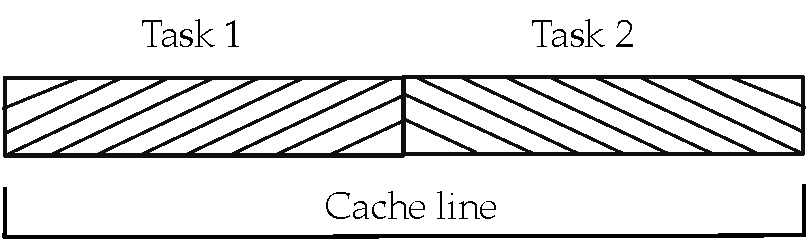
\includegraphics[width=2.4in]{figure/falsesharing}
}%
\hspace{30pt}
\subfigure[True sharing]{%
   \label{fig:tsinfs}
   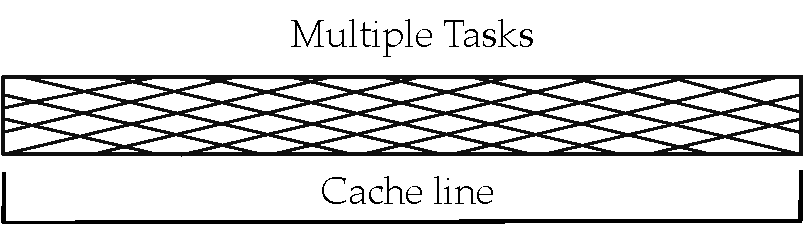
\includegraphics[width=2.4in]{figure/truesharing}
}%
\caption{False sharing (a) vs. true sharing (b). For false sharing, different tasks access different parts of the same cache line simultaneously. For true sharing, multiple tasks access the same part of a cache line.\label{fig:falsesharing}}
\end{figure}

Common programming practice can easily introduce false sharing. For an example shown in Figure~\ref{fig:penaltycode}, different threads access different words of the same global array, but involving in a big number of unnecessary cache invalidations. This problem is hard to find out manually by checking the results of executions.  

After the detection, there are several ways to fix them by preventing multiple threads from accessing the same cache line simultaneously. {\tt First},  we can pad useless words into a corresponding structure or class. {\tt Second}, we can assign the value of falsely-shared variable to a thread-local variable so that different threads may update their local variables, and commit those changes back to the shared variable in the end. {\tt Third},  some systems can isolate the execution of different threads, but with their own limitations on applications and the environment~\cite{Sheriff, OSdetection}. 
%However, Sheriff only works for multithreaded programs that are using the standard \pthreads{} library, without ad hoc synchronizations~\cite{Xiong:2010:AHS:1924943.1924955} and communication across the stack. 
Thus, mostly people are still using the first two approaches to fix false sharing problems by changing the code manually. For these approaches, programmers should have precise information about falsely-shared objects in order to fix them. \cheetah{} aims to provide precise information as much as possible, such as where are those falsely-shared objects, what is access pattern of memory accesses, and how much performance improvement after fixes. 


\sloppy
\subsection{Motivation of Efficient Memory Trace Collection}
Analyzing memory access patterns is an effective way to pinpoint false sharing. However, capturing memory accesses via software methods is costly, even with various sampling techniques~\cite{macpo,SLO2}. The overhead can be as high as 2-5$\times$, which is often not applicable to real applications working on large data sets and running in a highly threaded platform. Moreover, the high overhead leads to inaccurate measurement of program execution, which inconveniences the impact assessment of performance bottlenecks.

To address this issue, recent hardware performance monitoring units (PMU) support sampling memory accesses with extremely low overhead, less than 5\%. There are two typical sampling mechanisms in modern architectures: instruction-based sampling (IBS)~\cite{AMDIBS:07} supported in AMD Opteron processors and precise event-based sampling (PEBS) with load latency extension~\cite{IntelArch:PEBS:Sept09} in Intel Nehalem processors as well as their successors. Both IBS and PEBS can sparsely sample memory loads and stores at the same time. For each load sample, IBS and PEBS capture its effective address and the latency in CPU cycles from this sampled instruction issued to retired. For each store sample, IBS and PEBS capture its effective address only. Moreover, both IBS and PEBS record the precise instruction pointers of sampled memory accesses, which can be used to associate the analysis with program's source code. To make our analysis efficient, we build \Cheetah{} based on PMU sampling. 

 \subsection{Overview of Cheetah}

\begin{figure}[htbp]
\centering
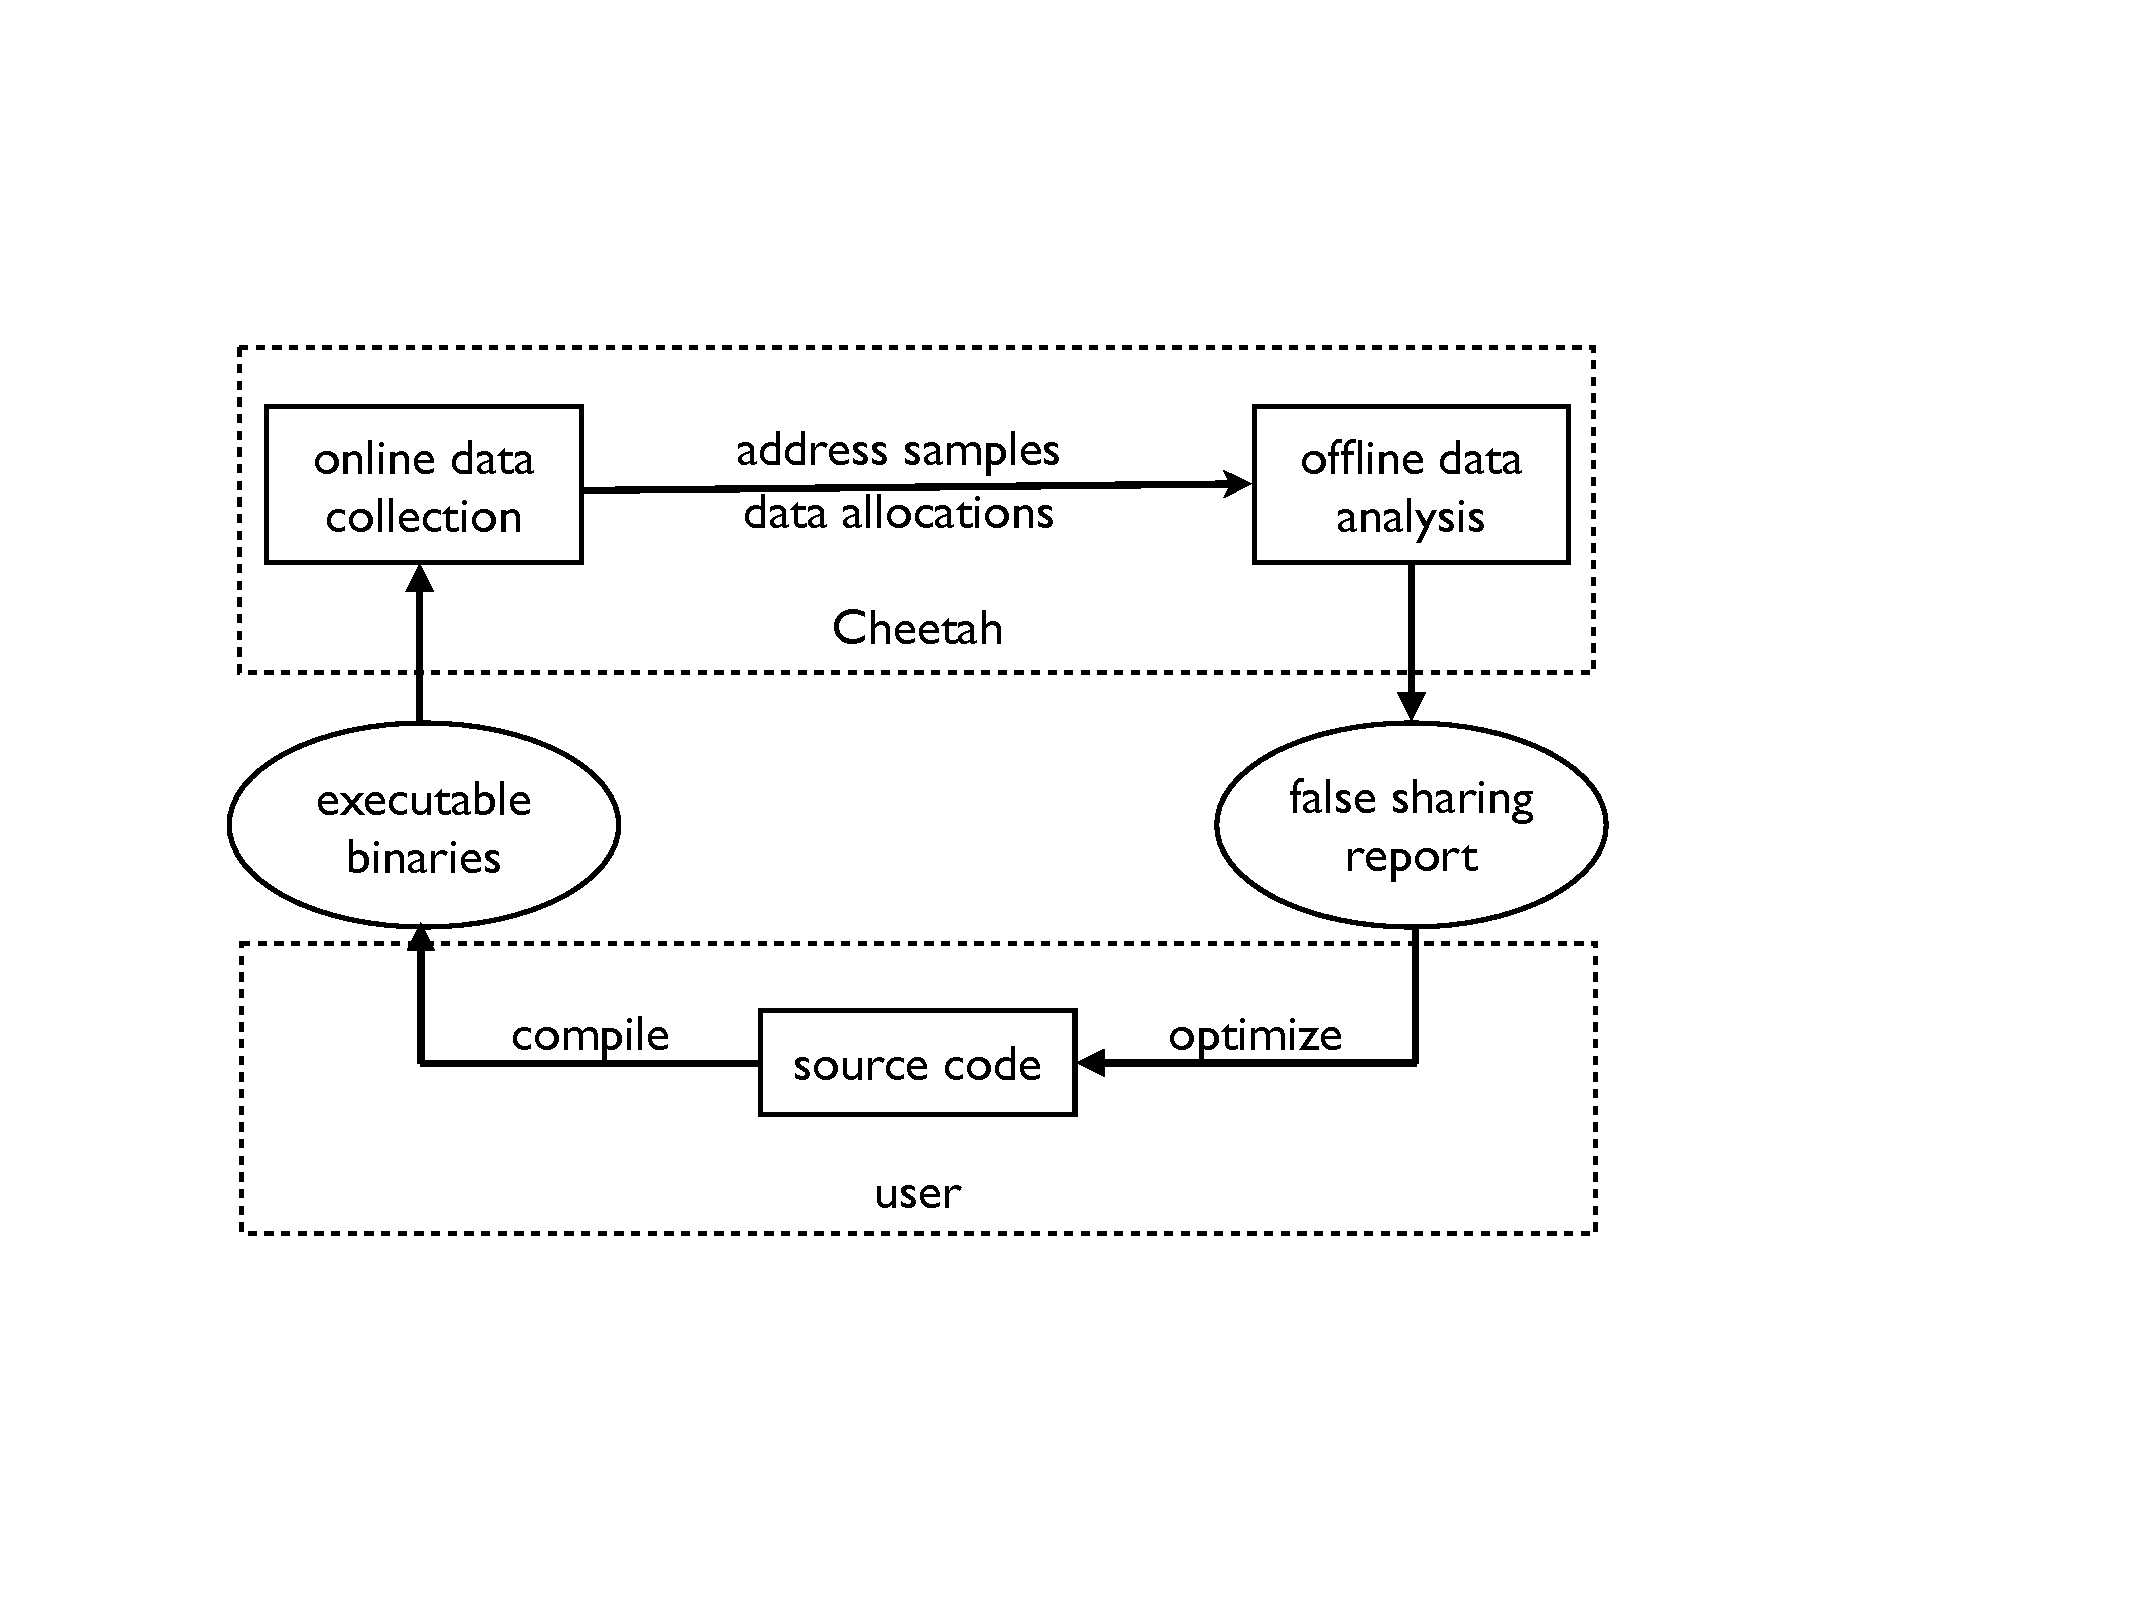
\includegraphics[width=\columnwidth]{figure/workflow}
\caption{The workflow of \cheetah{}.}
\label{fig:workflow}
\end{figure}

\Cheetah{}, as shown in Figure~\ref{fig:workflow}, consists of two components: an online profiler and an offline analyzer. The online profiler leverages PMU to monitor program execution and the offline analyzer processes all performance data collected by the profiler. Finally, \cheetah{} generates a report to guidance programmers for code optimization. 
To distinguish \cheetah{} from existing tools, we claim that \cheetah{} can detect false sharing efficiently and effectively. For its efficiency, \cheetah{} incurs low runtime overhead, around 10\%, which is much lower than the state-of-the-art tool, such as Predator~\cite{Predator}. For its effectiveness, \cheetah{} precisely identifies false sharing, without reporting any true sharing. Moreover, it provides detailed optimization guidance, including source code information, data object information, and assessment of improvement potentials.

In the following two sections, we elaborate how \cheetah{} efficiently detects false sharing and assesses its impact to the whole program execution.




\section{Detecting False Sharing}
\label{sec:detect}

% What is the basic idea? Why those ones uses performance counters can not reveal false sharing problems? 
\cheetah{} aims to report false sharing with significant performance impact. Since only cache lines with a large number of cache invalidations can have big performance impact on the performance, \cheetah{} should locate those cache lines. However, this task turns out to be difficult because cache invalidation depends on pattern of memory accesses, actual cache hierarchy and thread-to-core mappings. 

Thus, \cheetah{} proposes a simple rule to track cache invalidations: {\emph if a thread writes a cache line after other threads have accessed the same cache line, this write operation causes a cache invalidation}. This rule is based on the following two assumptions:
 
%Though hardware performance counters can collect events related to the cache invalidation, they have difficulties in identifying its root causes, such as instructions and data objects involved in the cache invalidation. In contrast, directly analyzing the memory traces collected by PMU can give more insights. Given a set of memory addresses, one typically needs the configuration of cache hierarchy and the knowledge of thread-to-core mappings to perform accurate analysis. 

\begin{itemize} 
\item {\bf Assumption 1:} Each thread runs on a separate core with its own private cache. 

\item {\bf Assumption 2: } Cache sizes are infinite. 
 
\end{itemize}

Assumption 1 is reasonable because thread over-subscription is generally rare for computation intensive programs. This assumption just over-reports the number of cache invalidations, if multiple threads are actually scheduled to the same core or different cores may share part of cache hierarchy. In this meaning, Assumption 1 actually presents the worst scenario for a given false sharing instance. With this assumption, \cheetah{} is independent from thread-to-core mapping or actual cache hierarchy.

Assumption 2 further defines the behavior related to cache eviction and invalidation. If there is a memory access within a cache line, the hardware cache (of running this thread) always holds the data until an access of other threads (running on other cores by assumption 1) invalidates it.  This assumption avoids to track cache evictions caused by cache capacity. 
%However, 
%If there is a memory access within a cache line, the hardware cache (of running this thread) always holds the data until an access of other threads (running on other cores by assumption 1) invalidates it. Thus, there is no need to track cache evictions that are caused by cache capacity. 

Combing these two assumptions, \cheetah{} can identify cache validations simply based on the pattern of memory accesses, without knowing the actual memory hierarchy and parallel execution environments. Based on this rule, we can report the number of cache validations by analyzing memory traces only, similar to the prior work~\cite{Predator, qinzhao}. 

In the remaining of this section, we elaborate how we install PMU-based sampling mechanism for memory accesses in Section~\ref{sec:perfcounter}, how we track memory accesses and data allocation in Section~\ref{sec:shadow}, how we analyze access patterns for cache invalidation in Section~\ref{sec:computeinvalidations}, and how we report false sharing in Section~\ref{sec:report}.
% This idea is similar to Predator. But Predator is a compiler-based approach, which needs to change the source code of applications. Also, it introduces much performance overhead that can block its use in deployment environment. 

% To reduce the performance overhead, 
% Basic idea, by examing the memory access pattern

\subsection{Memory Accesses Sampling}
\label{sec:perfcounter}

According to the basic rule described above, it is very important to track memory accesses of different threads in order to compute the number of cache invalidations on each cache line. 
%The state-of-the-art work \Predator{} leverages the compiler instrumentation to insert function calls before every memory access~\cite{Predator}. However, this approach introduces more than $5\times$ performance overhead by instrumenting every memory access. Moreover, \Predator{} has to re-compile applications, which needs the availability of source code. \Predator{} is not desirable for legacy applications without the source code, or real deployment that is sensitive to performance. 
\cheetah{} aims to significantly reduce the performance overhead by leveraging PMU-based sampling (i.e., AMD IBS and Intel PEBS), described in Section~\ref{sec:sampling}.
%hardware performance monitoring units (PMUs) that are available in most modern architectures. 
For each sample, PMU distinguishes whether it is a memory read or write, captures the memory address touched by the sampled memory access, and record the thread ID that triggers this sample. \Cheetah{} performs the analysis of false sharing based on these three pieces of information.3
%These information is enough to compute the number of cache invalidations based on the basic rule that is described in Section~\ref{sec:basicidea}. 
Since hardware performance counter only samples a memory access out of a specified number, it doesn't pose significant performance overhead. 
%Besides that, using performance counters does not need to instrument source code explicitly, thus providing a non-intrusive way to monitor memory references. 

{\color{blue}Do you want to put this section in the related work?}
\cheetah{} is different with existing approaches using hardware performance counters to detect false sharing problems~\cite{mldetect, openmp, detect:ptu}. Jayasena et. al. collects different types of events like memory accesses, data caches, TLBs, interactions among cores, and resources stalls, and derives potential memory patterns that can cause false sharing~\cite{mldetect}. DARWIN collects cache coherence events at the first round, then identifies possible memory accesses on those data structures that are involved in frequent cache invalidations for the second round~\cite{openmp}. DARWIN also requires manual effort or expertise to verify whether false sharing occurs or not.  Intel's PTU also relies on memory sampling mechanism but can not differentiate false sharing and true sharing since it discards the temporal information of memory accesses~\cite{detect:ptu}. More details on the difference have been discussed in Section~\ref{sec:relatedwork}.

\paragraph{Implementation} 
\cheetah{} intercepts process and thread creation by preloading its profiling library into the application address space without source code modification. Before executing any process or thread, \cheetah{} programs the PMU registers to turn on sampling with a pre-defined threshold. \cheetah{} also installs a signal handler to capture the sample in the form of interrupt signals in the user space. In order to guarantee the thread that triggers the interrupts can also captures them in the handler, 
%In order to sample memory accesses, \cheetah{} has to setup hardware registers before entering the \texttt{main} routine of the application.  \Cheetah{} installs a signal handler so that it can collect detailed information of memory accesses after a specified sample period. In order to simplify the signal handling, \Cheetah{} also configures the signal handler to be responded by the current thread, 
\cheetah{} sets \texttt{F\_SETOWN\_EX} flag when using \texttt{fcntl} function to bind signals with threads. \cheetah{} also sets up the custom allocator and its internal heap in the initialization.

Inside the signal handler, \Cheetah{} collects detailed information of every sampled memory access, including its memory address, thread id, read or write operation, and access latency, which can be fed into the computing module to compute the number of cache invalidations and the prediction module to predict performance impact.

\subsection{Shadow Memory and Customized Heap}
\label{sec:shadow}

For each sampled memory access, \cheetah{} has to locate its specific cache line so that we can compute the number of cache invalidations. \Cheetah{} utilizes the shadow memory mechanism to speedup the locating process. Shadow memory has been utilized extensively in different fields, such as detecting concurrency bugs~\cite{Harrow:2000:RCM:645880.672080, helgrind, 404681, Savage:1997:EDD:268998.266641}, tracking information flow or data flow~\cite{Cheng:2006:TEF:1157733.1157903, Newsome05dynamictaint, Qin:2006:LLP:1194816.1194834}, or detecting memory errors or others~\cite{qinzhao, Hastings91purify:fast, Seward:2005:UVD:1247360.1247362, Narayanasamy:2006:ALO:1140277.1140303}.  

To utilize the shadow memory mechanism, we should determine the range of heap memory, which is difficult to know beforehand if using the default heap. \cheetah{} built its custom heap based on Heap Layers~\cite{Berger:2001:CHM:378795.378821}. \cheetah{} pre-allocates a fixed size of memory
from its underlying operating system using \texttt{mmap} system calls and satisfies memory allocations from this block of memory. \cheetah{} also adapts the per-thread heap organization used by Hoard~\cite{Hoard} so that two objects in the same cache line will never be allocated to two different threads. This design prevents inter-objects false sharing, but also makes \cheetah{} can not report false sharing problems caused by the heap allocator.  However, we argue that this problem should be fixed by using a modern heap allocator like Hoard~\cite{Hoard}. 

\paragraph{Implementation} 
To use its custom heap, \cheetah{} intercepts all memory allocations and deallocations. \cheetah{} initializes the heap before the application enters into \texttt{main} routine, by putting the initialization routine into the constructor attribute. \cheetah{} maintains two different heaps, where all memory usage of the application will be satisfied from its application heap and other memory usage will be allocated from its  internal heap. For both heaps, \cheetah{} manages objects based on the unit of {\it power of two}. For each memory allocation from the application, \cheetah{} saves the information of callsite and size by adding an object header to each object. This helps \cheetah{} to precisely report the line information of falsely-shared objects.  

%heap and globals. 
%Two huge arrays. 
\cheetah{} keeps track of memory accesses of global variables and objects of the application heap using the shadow memory technique. \Cheetah{} allocates two large arrays (by using \texttt{mmap}) to keeping track of the number of writes and detailed access information on each cache line. For each memory address, \cheetah{} uses the bit shift to compute the index of cache line and locates the placement of its corresponding array quickly. 


\subsection{Computing Cache Invalidations}
\label{sec:computeinvalidations}

\Cheetah{} targets to report false sharing that can have performance impact on applications. \Cheetah{} focuses on those false sharing problems with a significant number of cache invalidations.  

Qin Zhao et. al. propose to compute the number of cache invalidations based on the ownership of cache lines: when a thread updates an object that it does not own, it will cause cache invalidations and set the owner to the current thread~\cite{qinzhao}. However, this approach cannot be easily to scalable to more than 32 threads because of excessive memory consumption, where every word with 32-bits can only tracking 32 threads. Also it introduce significant performance overhead by utilizing the dynamic instrumentation technique and maintaining ownership of different cache lines. 

To overcome these shortcomings, \Cheetah{} maintains a two-entries-table ($T$) for each cache line ($L$) that is borrowed from Predator~\cite{Predator}, where each entry tracks accesses from one thread in a period. \Cheetah{} also keeps a counter for every cache line that indicates the number of cache invalidations on this cache line.  
According to the basic rule that are described in Section~\ref{sec:basicidea}, only a write access can cause a cache invalidation. When there is a cache invalidation, the current write access will flush the table and will be added into its corresponding table ($T$). Thus, a table will always have an entry except in the beginning. More specifically, \cheetah{} checks possible cache invalidations as follows.
 
\begin{itemize}
\item
  For each read access $R$, \cheetah{} will check: 
  \begin{itemize}
    \item
      If $T$ is full, there is no need to record this read access.
    \item
      If $T$ is not full and the existing entry has a different thread ID, 
      then \cheetah{} records this read access by adding a new entry to the table.
  \end{itemize}
\item
  For each write access $W$,  
  \begin{itemize}
    \item
      If $T$ is full, then $W$ causes a cache invalidation since at least one of two existing entries are issued by another thread (on another core).
    \item
      If $T$ is not full (and not empty),
      \cheetah{} checks whether the current $W$ is from the same thread as the existing entry . If
      so, $W$ will not cause a cache invalidation. Otherwise, there is a cache invalidation caused by this $W$.
  \end{itemize}
\end{itemize}

      
In the end, \cheetah{} can collect the number of cache invalidations happened on each cache line. 

\paragraph{Implementation} 

When there is an memory access, \Cheetah{} checks against its two-entries-cache-history table for the current cache line and determines whether an access leads to a cache invalidation according to the rule discussed above. 

Since \cheetah{} only cares about those cache lines that can potentially involve in false sharing. We observe that only those cache lines with a big number of writes can possibly cause a lot of cache invalidations. Based on this observation, cache lines with a small number of writes are never be a target that can cause serious performance problem. For this reason, \Cheetah{} tracks  the number of writes on a cache line at first, and only tracks detailed information when this number is larger than a pre-defined threshold, which we refer to as the {\it Tracking-Threshold}. To save memory, \cheetah{} only allocates memory to record the detailed information for all words in this cache line after this threshold.
 
After this threshold is reached, \Cheetah{} will track detailed read/write information for each access: what the address of an access; whether this is a read or write access; which thread issues this access. These information are going to be checked in the reporting phase that is described in Section~\ref{sec:report}. 

 \subsection{Reporting False Sharing}
% How we will report false sharing precisely and correctly?
% How we 
\label{sec:report}

\Cheetah{} aims to report false sharing correctly and precisely, same as existing work~\cite{Sheriff, Predator}. \Cheetah{} will invoke the process of checking and reporting false sharing problems, either at the end of programs or receiving the instructions from users through the \texttt{SIGUSR2} signal.  

\paragraph{Correct Detection} \Cheetah{} keeps track of word-based (four bytes) memory accesses on susceptible cache lines: how many reads or writes occurs by which thread on each word. When more than one thread access a word, \Cheetah{} marks this word to be shared. By identifying accesses on each word on a susceptible cache line, we can easily differentiate false sharing from true sharing, as shown in Figure~\ref{fig:falsesharing}. Word-based information can also help diagnose false sharing problems in more detail, which helps programmers to decide how to padding an existing data structure in order to avoid false sharing. Because it is possible for a thread, particularly the main thread, to allocate an object and do some initialization before passing to different threads,  \cheetah{} only tracks the information of memory accesses inside parallel phases to avoid this problem.

\paragraph{Precise Detection} \Cheetah{} reports precise information for global variables and heap objects that are involved in false sharing. For global variables, \Cheetah{} reports names and addresses by searching through the ELF symbol table. For heap objects, \Cheetah{} reports the lines of code for allocating these objects.  
Thus, \Cheetah{} intercepts all memory allocations and de-allocations and utilizes \texttt{backtrace()} to obtain the whole callsite stack. 
%During the real implementation, we tried to keep the overhead of getting the callsite stack as little as possible. \cheetah{} utilizes a global hash table to save those known callsite stack. The combination of ``rip'' (instruction pointer) and ``stack offset'' is considered as the key of this global hash table. If the combination of these two values (as the key) have existed in the global hash table, we simply copied the saved callsite stack to a new object. Otherwise, backtrace() is called to fetch the callstack.  

 
%\cheetah{} only reports those false sharing problems that can have a significant impact on the performance by predicting the upper bound of performance improvement, according to the idea that are discussed in Section~\ref{sec:predictidea}.  It will rank the severity of performance degradation of any detected false sharing problems based on the predicted performance improvement after fixes.

%\section{Predicting Performance Impact}
\section{Assessing the Performance Impact}

\label{sec:predictimprove}

Fixing false sharing problems can be non-trivial, even with precise information about a particular false sharing problem. However, fixing false sharing problems does not necessarily bring the performance improvement. For example, existing tools report a big number of cache invalidations that are caused by false sharing in word\_count or reverse\_index applications, but fixing them brings negligible performance improvement~\cite{Sheriff, Predator}. Zhao et. al. observed that fixing may even slowdown a program because of excessive memory consumption or the lose of locality~\cite{qinzhao}. Reporting insignificant false sharing instances are not false positives, but that increases manual burden for programmers.

To resolve this problem, \cheetah{} makes the first attempt to quantitatively assess the potential performance gain of fixing a particular false sharing problem. So that programmers can focus on severe problems only, avoiding unnecessary manual effort.

Assessing the performance impact is a very challenging topic. \todo{Currently we do not find much related work~\cite{}, not to mention the impact of false sharing problems}. False sharing occurs when more than two threads are accessing the same cache line. Thus, to assess the performance impact of false sharing problems, we have to monitor the execution of different threads. For example, if a thread is not in the critical path of the performance, then fixing false sharing problems in this thread will not have an observed impact on the final performance. The assessment can become even more complicated if there are some nested threads in the application.

To simplify our prediction and verify the idea, \cheetah{} focuses on its assessment on the normal fork-join model, which is the most important and widely used model. A basic example of fork-join model is shown in  Figure~\ref{fig:forkjoinmodel}. All applications that we evaluated in this paper, including all benchmarks in phoenix and parsec benchmarks suite, utilizes this fork-join model. 

\begin{figure*}[ht!]
\begin{center}
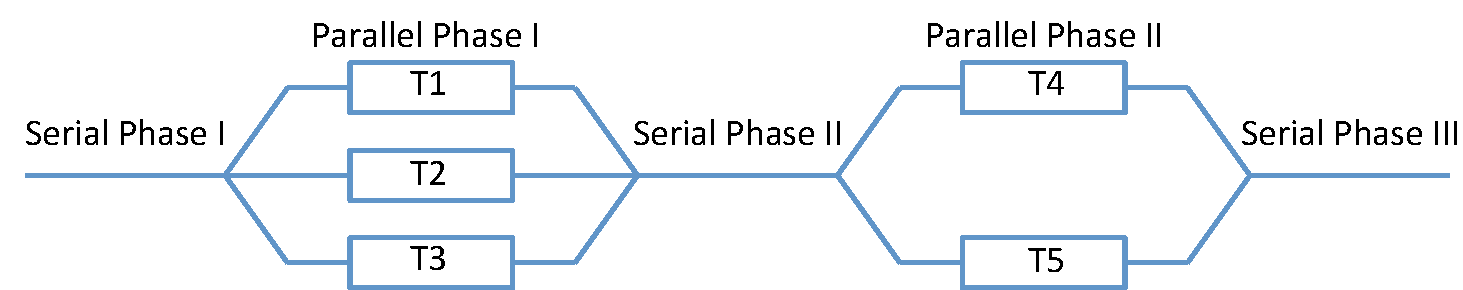
\includegraphics[width=6.5in]{figure/forkjoin}
\end{center}
\caption{\Cheetah{} assesses the impact of false sharing instances of applications with the fork-join model.
\label{fig:forkjoinmodel}}
\end{figure*}

\cheetah{} predicts the impact of an falsely-shared object $O$ on the application into three steps as follows. 

\begin{itemize}
\item \cheetah{} first evaluates how much , which is discussed in Section~\ref{object}. 
\item Then we discuss on the 
\item
\end{itemize}


%Why? The execution of different threads? Performance are closely related to a lot of events, such as cache uses, scheduling, thread-core affinity, locality. Our attempts is just the first try to give some upper bound.  For example, ~\cite{qinzhao} paper. 

But we will try to resolve this and evaluate the precision of our assessment in Section~\ref{}. 

Since we already know this situation, \cheetah{} currently focuses on the widely used and most important execution model -- fork-join model. All applications evelauted .. 


To assess 

These two questions are actually hard to answer, without knowing the running situations of different threads. 





\subsection{Impact on Accesses of this Object}

\subsection{Impact on Related Threads}

\subsection{Impact on the Application}

\subsection{Basic Idea}

\cheetah{}'s assessment is based on the following observations:

\begin{itemize}
\item we can use the results of sampling to represent the whole execution because sampling is evenly distributed over the whole execution. Based on the similar observation, exiting work like Oprofile and Gprof uses the sampling technique to identify the hotspots of function calls and code~\cite{oprofile, DBLP:conf/sigplan/GrahamKM82}.

\item PMU hardware provides the latency information (e.g. cycles) of each memory load operation. We also observed that the latency of accessing falsely shared objects is significantly higher than that of normal accesses. 

\end{itemize}

Based on these two observations, {\bf we propose to use the sampled cycles of an execution to represent the execution time or the runtime}. \cheetah{} will compute the performance improvement based on EQ.(\ref{eq:improvement}), where runtime is denoted by $RT$.
\begin{equation}
\label{eq:improvement}
Perf_{improve}=RT_{actual}/RT_{predict}
\end{equation}


%Thus, based on this equation, the most important thing is to compute $RT_{predict}$, which can be represented by the cycles of accesses after fixing a false sharing instance. $RT_{actual}$ can represented by the sampled cycles of accesses.

%Although it is impossible to know the exact cycles after fixing a false sharing instance, we can estimate based on our two observations as follows. 

To assess the performance impact of a falsely-shared object $O$, \cheetah{} has to collect the following information. 
 
\begin{itemize}
\item $Cycles\_O$: total cycles on a falsely-shared object $O$.
\item $Accesses\_O$: total number of accesses on the object $O$.  
\item $AverageCycles\_{nofs}$: the average cycles of every memory access on non-falsely-shared (abbreviated as ``non-FS'') objects. \cheetah{} utilizes the average cycles of each access that happened in the serial phases as the $AverageCycles\_{nofs}$. There is no false sharing problem in serial phases since there is only one thread in total.  

\end{itemize}

Based on EQ.(\ref{eq:improvement}), we compute the potential performance improvement as EQ.(\ref{eq:improvement2}). Here, we utilize $Cycles\_O$ to represent $RT_{actual}$, while  $RT_{predict}$ can be represented by the product of $Accesses\_O$ and $AverageCycles\_{nofs}$. For $RT_{predict}$ , we assume that the number of accesses after fixing keeps the same (e.g. $Accesses\_O$), and the best latency of each access after fixing the false sharing problem of the object $O$ will be equal to $AverageCycles\_{nofs}$. {\bf This is the basic idea of \cheetah{}'s assessment}. 

\begin{equation}
\label{eq:improvement2}
 Perf_{improve}= Cycles\_O/(AverageCycles\_{nofs} * Accesses\_O);
\end{equation} 



% Now we are going to discuss how to utilize this idea to actually compute the performance of multithreaded programs.  

% How to predict the runtime after fixing false sharing. We are 
% using the cycles of non-fs objects and fs-objects. 
% the number of accesses, and the total number of cycles of fs objects. 

The EQ.(\ref{eq:improvement2}) tells the performance improvement of accesses on a false sharing object. But our final target is know the improvement of the  application itself by fixing a false sharing instance inside. To achieve the final target, we have to compute the following two more things:

\begin{itemize}
\item How much performance improvement each involved thread can get by fixing this instance?

\item How much performance improvement the total application can get by fixing this instance? 

\end{itemize}

These two questions are actually hard to answer, without knowing the running situations of different threads. For example, if a thread is not in the critical path of the performance, then fixing false sharing problems in this thread will not have an explicit impact on the final performance. The assessment can become even more complicated if there are some nested threads in the application. 

To approve the basic concept, 
%\cheetah{} collects the execution information on different phases, different threads, and different objects. 

This section will present the details of \cheetah{}'s prediction. We first describe the general idea using the Figure~\ref{fig:forkjoinmodel} as an example. In this example, only thread $T1$ and $T2$ are involved in a falsely-shared object $O$, \cheetah{} has to know the following information:

 

\subsection{Collecting Execution Information}
\label{sec:getactualtime}

\paragraph{Threads Model Information:} For fork-join models, only the main/initial thread can perform spawning operations. It is easy to verify this by intercepting spawning functions, such as the \texttt{pthread\_create} functions of programs using the \texttt{pthreads} library. 

\paragraph{Phase information:} \Cheetah{} collects the execution time of different serial and parallel phases using RDTSC (ReaD-Time Stamp Counter) on X86 machines.  The difference between the stopping point and the starting point will be considered as the length of a phase. It is relatively easy for \cheetah{} to collect the length of serial phases since \cheetah{} intercepts the spawning operations. For the same reason, \cheetah{} gets the timestamps of the starting point and the stopping point of each thread, then uses the longest span of each thread as the length of every parallel phase. \Cheetah{} also tracks the number of accesses and the cycles of every accesses in serial phases. It uses the average cycles of every memory access in serial phases to be the $Cycles\_{nofs}$ discussed above.  
 
\paragraph{Threads Information:} \Cheetah{} collects the following information of different threads: execution time, number of accesses, and number of cycles of all memory accesses. 

\paragraph{Objects Information:}
For each cache line, \cheetah{} gathers the number of cycles on each cache line. \cheetah{} also collect the number of accesses on each word. Thus, we can compute the number of cycles and accesses on falsely-shared objects. 
 
\subsection{Predicting Execution Time after Fixes}
\label{sec:predicttime}

\cheetah{} predicts the execution time after fixes by replacing the actual cycles of every memory access on a falsely-shared object with the average cycles of a memory access without false sharing. 

According to this, \cheetah{} should know the average cycles of a memory access without false sharing and true sharing. \Cheetah{} actually utilizes the cycles of every memory access in serial phases (denoted as $Cycles_{nofs}$) to approximate this value, which is reasonable since all memory accesses in serial phases should not involve in both false sharing and true sharing. 

Actual cycles of every memory access that are involving in a falsely-shared object can be changed from one execution to another. Thus, \cheetah{} utilizes the total number of all memory accesses instead to predict the performance impact. \Cheetah{} computes the possible performance improvement prediction in the following steps.
 
\begin{enumerate}
\item \cheetah{} first compute the total number of accesses ($Accesses_{fs}$) on suspected cache lines and the total cycles of accesses ($Cycles_{fs}$) on suspected cache lines.

\item For threads that are involved a particular false sharing, \cheetah{} then compute the total number of accesses ($Accesses_{threads}$) and the total cycle of accesses ($Cycles_{threads}$). 

\item \Cheetah{} computes the estimated cycles of those threads that are involved in false sharing according to the formula $Cycles_{pred} = Cycles_{threads} - Cycles_{fs} + Accesses_{fs} * AverageCycles_{nofs}$. 

\item  Based on this, \cheetah{} will compute the performance improvement on threads that are involved in false sharing.
$RT_{threads} = Cycles_{threads}  $. 

\end{enumerate}



\cheetah{} will utilize the latency information of every access to predict the performance impact of a certain false sharing instance. These latency information, normally CPU cycles of every sampled memory access, can be provided by hardware PMUs. \Cheetah{} plans to track detailed memory accesses on falsely-shared objects and on normal objects without false sharing. Thus, we can know the average cycles of every memory access without false sharing. 

\cheetah{} provides a upper bound on performance improvement after fixes. 

It is note that sampling based approaches can actually 
.

We only compute the cycles and threads for the parallel phases. 

\subsection{Predicting Performance Improvement}

Using the $ImproveRate$, we can compute the possible runtime of $T1$ and $T2$ after fixing the false sharing problem of object $O$, which are equal to the product of the actual runtime and $ImproveRate$. If the computed runtime is less than the length of $T3$ in parallel phase I, fixing the false sharing problem of object $O$ won't contribute any performance improvement of the program. Otherwise, it can benefit the performance. Then we compute the new runtime of parallel phase I, which equals to the longest runtime of thread $T1$, $T2$ or $T3$. Based on this, we computes the new runtime of this program, where the execution time of other phases should not be affected. In the end, \cheetah{} predicts the possible performance rate of fixing every false sharing problem so that programs can focus on those important problems.
%There are several steps to evaluate the performance impact. We will consider the average cycles on every access in serial phases as $Cycles_{serial}$. 

 % How to avoid huge performance overhead? We introducing per-thread recording mechanism. 

% How to actually predict the performance improvement? A thread may have the serial part and parallel part. We have to identify the serial part and parallel part. 

% How to handle different CPUs? For example, we may start 16 threads on 8 CPUs. 

% Can we get the resolute time on each phase? We are using this to calculate the performance improvement.  We also copy the whole memory accesses information out before transferring phases. 

% What if only two threads only accesses a specific cache line and other threads didn't accesses that? We can actually check the word level's accesses to find out those number of threads that are accesses this tid. We could also verify whether those memory accesses are on the critical path or not. 

% We should use actual tid instead of thread index to identify threads. 

% We should remove the write-invoked tracking since we have to check the number of accesses. Thus, we actually don't care those ones that are happened in the serial phase. Because we won't actual change its performance initially. 



% The total number of memory accesses on an addresses

% The total latency of accessing an address

% The total number of memory accesses for each thread. 

% The total latency of all memory accesses for each thread  

% All memory accesses of each thread

% All memory accesses in total = Sum of (memory accesses of each thread)

% Total latency of all memory accesses for each thread. 

%\section{Predicting Performance Impact}
%\section{Assessing the Performance Impact}

\label{sec:predictimprove}

Fixing false sharing problems can be non-trivial, even with precise information about a particular false sharing problem. However, fixing false sharing problems does not necessarily bring the performance improvement. For example, existing tools report a big number of cache invalidations that are caused by false sharing in word\_count or reverse\_index applications, but fixing them brings negligible performance improvement~\cite{Sheriff, Predator}. Zhao et. al. observed that fixing may even slowdown a program because of excessive memory consumption or the lose of locality~\cite{qinzhao}. Reporting insignificant false sharing instances are not false positives, but that increases manual burden for programmers.

To resolve this problem, \cheetah{} makes the first attempt to quantitatively assess the potential performance gain of fixing a particular false sharing problem. So that programmers can focus on severe problems only, avoiding unnecessary manual effort.

Assessing the performance impact is a very challenging topic. \todo{Currently we do not find much related work~\cite{}, not to mention the impact of false sharing problems}. False sharing occurs when more than two threads are accessing the same cache line. Thus, to assess the performance impact of false sharing problems, we have to monitor the execution of different threads. For example, if a thread is not in the critical path of the performance, then fixing false sharing problems in this thread will not have an observed impact on the final performance. The assessment can become even more complicated if there are some nested threads in the application.

To simplify our prediction and verify the idea, \cheetah{} focuses on its assessment on the normal fork-join model, which is the most important and widely used model. A basic example of fork-join model is shown in  Figure~\ref{fig:forkjoinmodel}. All applications that we evaluated in this paper, including all benchmarks in phoenix and parsec benchmarks suite, utilizes this fork-join model. 

\begin{figure*}[ht!]
\begin{center}
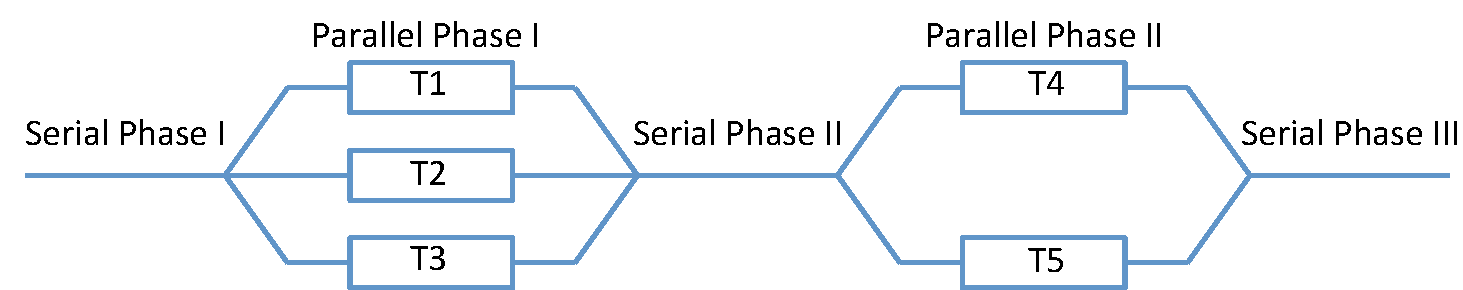
\includegraphics[width=6.5in]{figure/forkjoin}
\end{center}
\caption{\Cheetah{} assesses the impact of false sharing instances of applications with the fork-join model.
\label{fig:forkjoinmodel}}
\end{figure*}

\cheetah{} predicts the impact of an falsely-shared object $O$ on the application into three steps as follows. 

\begin{itemize}
\item \cheetah{} first evaluates how much , which is discussed in Section~\ref{object}. 
\item Then we discuss on the 
\item
\end{itemize}


%Why? The execution of different threads? Performance are closely related to a lot of events, such as cache uses, scheduling, thread-core affinity, locality. Our attempts is just the first try to give some upper bound.  For example, ~\cite{qinzhao} paper. 

But we will try to resolve this and evaluate the precision of our assessment in Section~\ref{}. 

Since we already know this situation, \cheetah{} currently focuses on the widely used and most important execution model -- fork-join model. All applications evelauted .. 


To assess 

These two questions are actually hard to answer, without knowing the running situations of different threads. 





\subsection{Impact on Accesses of this Object}

\subsection{Impact on Related Threads}

\subsection{Impact on the Application}

\subsection{Basic Idea}

\cheetah{}'s assessment is based on the following observations:

\begin{itemize}
\item we can use the results of sampling to represent the whole execution because sampling is evenly distributed over the whole execution. Based on the similar observation, exiting work like Oprofile and Gprof uses the sampling technique to identify the hotspots of function calls and code~\cite{oprofile, DBLP:conf/sigplan/GrahamKM82}.

\item PMU hardware provides the latency information (e.g. cycles) of each memory load operation. We also observed that the latency of accessing falsely shared objects is significantly higher than that of normal accesses. 

\end{itemize}

Based on these two observations, {\bf we propose to use the sampled cycles of an execution to represent the execution time or the runtime}. \cheetah{} will compute the performance improvement based on EQ.(\ref{eq:improvement}), where runtime is denoted by $RT$.
\begin{equation}
\label{eq:improvement}
Perf_{improve}=RT_{actual}/RT_{predict}
\end{equation}


%Thus, based on this equation, the most important thing is to compute $RT_{predict}$, which can be represented by the cycles of accesses after fixing a false sharing instance. $RT_{actual}$ can represented by the sampled cycles of accesses.

%Although it is impossible to know the exact cycles after fixing a false sharing instance, we can estimate based on our two observations as follows. 

To assess the performance impact of a falsely-shared object $O$, \cheetah{} has to collect the following information. 
 
\begin{itemize}
\item $Cycles\_O$: total cycles on a falsely-shared object $O$.
\item $Accesses\_O$: total number of accesses on the object $O$.  
\item $AverageCycles\_{nofs}$: the average cycles of every memory access on non-falsely-shared (abbreviated as ``non-FS'') objects. \cheetah{} utilizes the average cycles of each access that happened in the serial phases as the $AverageCycles\_{nofs}$. There is no false sharing problem in serial phases since there is only one thread in total.  

\end{itemize}

Based on EQ.(\ref{eq:improvement}), we compute the potential performance improvement as EQ.(\ref{eq:improvement2}). Here, we utilize $Cycles\_O$ to represent $RT_{actual}$, while  $RT_{predict}$ can be represented by the product of $Accesses\_O$ and $AverageCycles\_{nofs}$. For $RT_{predict}$ , we assume that the number of accesses after fixing keeps the same (e.g. $Accesses\_O$), and the best latency of each access after fixing the false sharing problem of the object $O$ will be equal to $AverageCycles\_{nofs}$. {\bf This is the basic idea of \cheetah{}'s assessment}. 

\begin{equation}
\label{eq:improvement2}
 Perf_{improve}= Cycles\_O/(AverageCycles\_{nofs} * Accesses\_O);
\end{equation} 



% Now we are going to discuss how to utilize this idea to actually compute the performance of multithreaded programs.  

% How to predict the runtime after fixing false sharing. We are 
% using the cycles of non-fs objects and fs-objects. 
% the number of accesses, and the total number of cycles of fs objects. 

The EQ.(\ref{eq:improvement2}) tells the performance improvement of accesses on a false sharing object. But our final target is know the improvement of the  application itself by fixing a false sharing instance inside. To achieve the final target, we have to compute the following two more things:

\begin{itemize}
\item How much performance improvement each involved thread can get by fixing this instance?

\item How much performance improvement the total application can get by fixing this instance? 

\end{itemize}

These two questions are actually hard to answer, without knowing the running situations of different threads. For example, if a thread is not in the critical path of the performance, then fixing false sharing problems in this thread will not have an explicit impact on the final performance. The assessment can become even more complicated if there are some nested threads in the application. 

To approve the basic concept, 
%\cheetah{} collects the execution information on different phases, different threads, and different objects. 

This section will present the details of \cheetah{}'s prediction. We first describe the general idea using the Figure~\ref{fig:forkjoinmodel} as an example. In this example, only thread $T1$ and $T2$ are involved in a falsely-shared object $O$, \cheetah{} has to know the following information:

 

\subsection{Collecting Execution Information}
\label{sec:getactualtime}

\paragraph{Threads Model Information:} For fork-join models, only the main/initial thread can perform spawning operations. It is easy to verify this by intercepting spawning functions, such as the \texttt{pthread\_create} functions of programs using the \texttt{pthreads} library. 

\paragraph{Phase information:} \Cheetah{} collects the execution time of different serial and parallel phases using RDTSC (ReaD-Time Stamp Counter) on X86 machines.  The difference between the stopping point and the starting point will be considered as the length of a phase. It is relatively easy for \cheetah{} to collect the length of serial phases since \cheetah{} intercepts the spawning operations. For the same reason, \cheetah{} gets the timestamps of the starting point and the stopping point of each thread, then uses the longest span of each thread as the length of every parallel phase. \Cheetah{} also tracks the number of accesses and the cycles of every accesses in serial phases. It uses the average cycles of every memory access in serial phases to be the $Cycles\_{nofs}$ discussed above.  
 
\paragraph{Threads Information:} \Cheetah{} collects the following information of different threads: execution time, number of accesses, and number of cycles of all memory accesses. 

\paragraph{Objects Information:}
For each cache line, \cheetah{} gathers the number of cycles on each cache line. \cheetah{} also collect the number of accesses on each word. Thus, we can compute the number of cycles and accesses on falsely-shared objects. 
 
\subsection{Predicting Execution Time after Fixes}
\label{sec:predicttime}

\cheetah{} predicts the execution time after fixes by replacing the actual cycles of every memory access on a falsely-shared object with the average cycles of a memory access without false sharing. 

According to this, \cheetah{} should know the average cycles of a memory access without false sharing and true sharing. \Cheetah{} actually utilizes the cycles of every memory access in serial phases (denoted as $Cycles_{nofs}$) to approximate this value, which is reasonable since all memory accesses in serial phases should not involve in both false sharing and true sharing. 

Actual cycles of every memory access that are involving in a falsely-shared object can be changed from one execution to another. Thus, \cheetah{} utilizes the total number of all memory accesses instead to predict the performance impact. \Cheetah{} computes the possible performance improvement prediction in the following steps.
 
\begin{enumerate}
\item \cheetah{} first compute the total number of accesses ($Accesses_{fs}$) on suspected cache lines and the total cycles of accesses ($Cycles_{fs}$) on suspected cache lines.

\item For threads that are involved a particular false sharing, \cheetah{} then compute the total number of accesses ($Accesses_{threads}$) and the total cycle of accesses ($Cycles_{threads}$). 

\item \Cheetah{} computes the estimated cycles of those threads that are involved in false sharing according to the formula $Cycles_{pred} = Cycles_{threads} - Cycles_{fs} + Accesses_{fs} * AverageCycles_{nofs}$. 

\item  Based on this, \cheetah{} will compute the performance improvement on threads that are involved in false sharing.
$RT_{threads} = Cycles_{threads}  $. 

\end{enumerate}



\cheetah{} will utilize the latency information of every access to predict the performance impact of a certain false sharing instance. These latency information, normally CPU cycles of every sampled memory access, can be provided by hardware PMUs. \Cheetah{} plans to track detailed memory accesses on falsely-shared objects and on normal objects without false sharing. Thus, we can know the average cycles of every memory access without false sharing. 

\cheetah{} provides a upper bound on performance improvement after fixes. 

It is note that sampling based approaches can actually 
.

We only compute the cycles and threads for the parallel phases. 

\subsection{Predicting Performance Improvement}

Using the $ImproveRate$, we can compute the possible runtime of $T1$ and $T2$ after fixing the false sharing problem of object $O$, which are equal to the product of the actual runtime and $ImproveRate$. If the computed runtime is less than the length of $T3$ in parallel phase I, fixing the false sharing problem of object $O$ won't contribute any performance improvement of the program. Otherwise, it can benefit the performance. Then we compute the new runtime of parallel phase I, which equals to the longest runtime of thread $T1$, $T2$ or $T3$. Based on this, we computes the new runtime of this program, where the execution time of other phases should not be affected. In the end, \cheetah{} predicts the possible performance rate of fixing every false sharing problem so that programs can focus on those important problems.
%There are several steps to evaluate the performance impact. We will consider the average cycles on every access in serial phases as $Cycles_{serial}$. 

 % How to avoid huge performance overhead? We introducing per-thread recording mechanism. 

% How to actually predict the performance improvement? A thread may have the serial part and parallel part. We have to identify the serial part and parallel part. 

% How to handle different CPUs? For example, we may start 16 threads on 8 CPUs. 

% Can we get the resolute time on each phase? We are using this to calculate the performance improvement.  We also copy the whole memory accesses information out before transferring phases. 

% What if only two threads only accesses a specific cache line and other threads didn't accesses that? We can actually check the word level's accesses to find out those number of threads that are accesses this tid. We could also verify whether those memory accesses are on the critical path or not. 

% We should use actual tid instead of thread index to identify threads. 

% We should remove the write-invoked tracking since we have to check the number of accesses. Thus, we actually don't care those ones that are happened in the serial phase. Because we won't actual change its performance initially. 



% The total number of memory accesses on an addresses

% The total latency of accessing an address

% The total number of memory accesses for each thread. 

% The total latency of all memory accesses for each thread  

% All memory accesses of each thread

% All memory accesses in total = Sum of (memory accesses of each thread)

% Total latency of all memory accesses for each thread. 

%\section{\doubletake{} for Multithreading Programs}
%\input{multithreading}

%\section{Optimization}
%\input{optimization}
%\section{Implementation Details}
\label{sec:implement}





\begin{comment}


This section presents the detailed implementation of \Cheetah{}'s detection: it first describes how to sample memory accesses (in Section~\ref{sec:detect-trace}) and how to compute the number of cache invalidations based on the pattern of memory accesses (see Section~\ref{sec:compute}); then we describes how to report false sharing precisely and correctly (see Section~\ref{sec:report});

%\redmark{Should we add a figure about different components??}

\subsection{Sampling Memory Accesses}
\label{sec:detect-trace}
% How to trace the memory accesses?
% What is the benefit of using performance counter, non-instrusive
% What information that we can get about an memory access
% How we will handle this information? We will pass it to cache invalidations module

As described in Section~\ref{sec:perfcounter}, \Cheetah{} relies on hardware performance counters, such as AMD's IBS registers, to sample memory accesses. Hardware performance counters provide a non-intrusive and efficient approach to track memory accesses. \Cheetah{} is a library that can be preloaded before the execution of an application: there is no need to change or recompile the programs, or to modify the underlying operating system. 

\cheetah{} performs its initialization before running an application, by putting it into the constructor attribute. During the initialization, \Cheetah{} installs a signal handler so that it can collect detailed information of memory accesses after a specified sample period. In order to simplify the signal handling, \Cheetah{} also configures the signal handler to be responded by the current thread, by calling \texttt{fcntl} function with \texttt{F\_SETOWN\_EX} flag. \cheetah{} also sets up the custom allocator and its internal heap in the initialization.  

Inside the signal handler, \Cheetah{} collects detailed information of every sampled memory access, including memory address, thread id, read or write operation, and access latency, which can be fed into the computing module to compute the number of cache invalidations and the prediction module to predict performance impact. 

\subsection{Computing Cache Invalidations}
\label{sec:compute}

\Cheetah{} computes possible cache invalidations on each cache line based on the rule that is described in Section~\ref{sec:computeinvalidations}. \Cheetah{} maintains a two-entries-cache-history table for each cache line and checks against the history table to decide whether an access leads to a cache invalidation. In order to locate the cache history of each cache line, \Cheetah{} implements the shadow memory for all virtual addresses, which has been introduced before~\cite{qinzhao}. 

Since \cheetah{} only cares about those cache lines that can potentially involve in false sharing. We observe that only those cache lines with a big number of writes can possibly cause a lot of cache invalidations. Based on this observation, cache lines with a small number of writes are never be a target that can cause serious performance problem. For this reason, \Cheetah{} only tracks those cache lines when the number of writes on a cache line is larger than a pre-defined threshold, which we refer to as the {\it Tracking-Threshold}. Before this threshold is reached, \Cheetah{} only tracks the number of writes on a cache line while skipping tracking reads. This mechanism reduces performance and memory overhead at the same time.

In the implementation, \Cheetah{} maintains two arrays in the shadow memory: {\it CacheWrites} tracks the number of memory writes on every cache line, and {\it CacheTracking} tracks detailed information for each cache line. To save memory, {\it CacheTracking} for a particular cache line is allocated dynamically once the number of writes on this cache line exceeds the {\it Tracking-Threshold}. The history table, number of cache invalidations on a cache line, and detailed memory accesses are actually included in {\it CacheTracking}. These information are going to be checked in the reporting phase that is described in Section~\ref{sec:report}.
 
 \subsection{Reporting False Sharing}
% How we will report false sharing precisely and correctly?
% How we 
\label{sec:report}

\Cheetah{} aims to report false sharing correctly and precisely, same as existing work~\cite{sheriff, Predator}. \Cheetah{} will invoke the process of checking and reporting false sharing problems, either at the end of programs or receiving the instructions from users through the \texttt{SIGUSR2} signal.  

\paragraph{Correct Detection:} \Cheetah{} keeps track of word-based (four bytes) memory accesses on susceptible cache lines: how many reads or writes occurs by which thread on each word. When more than one thread access a word, \Cheetah{} marks this word to be shared. By identifying accesses on each word on a susceptible cache line, we can easily differentiate false sharing from true sharing, as shown in Figure~\ref{fig:falsesharing}. Word-based information can also help diagnose false sharing problems more detailed, which helps programmers to decide how to padding an existing data structure in order to avoid false sharing.  Because it is possible for a thread, particularly the main thread, to allocate an object and do some initialization before passing to different threads,  \cheetah{} only checks memory access inside parallel phases to avoid this problem.

\paragraph{Precise Detection.} \Cheetah{} reports precise information for global variables and heap objects that are involved in false sharing. For global variables, \Cheetah{} reports names and addresses by searching through the ELF symbol table. For heap objects, \Cheetah{} reports the lines of code for allocating these objects.  
Thus, \Cheetah{} intercepts all memory allocations and de-allocations and utilizes \texttt{backtrace()} to obtain the whole callsite stack. During the real implementation, we tried to keep the overhead of getting the callsite stack as little as possible. \cheetah{} utilizes a global hash table to save those known callsite stack. The combination of ``rip'' (instruction pointer) and ``stack offset'' is considered as the key of this global hash table. If the combination of these two values (as the key) have existed in the global hash table, we simply copied the saved callsite stack to a new object. Otherwise, backtrace() is called to fetch the callstack.  

\end{comment}
%However, it is straightforward to solve such false sharing problems by using an allocator like Hoard that avoids this kind of false sharing.


%\subsection{Predicting False Sharing}
% What is the basic idea to predict false sharing problem?
% What is the difference with Predator{}?
% For those predicted false sharing, we cannot predict performance improvement?



 

\section{Evaluation}
\label{sec:eval}

\sloppy{}
The evaluation answers the following research questions in order as follows. 

\begin{itemize}
\item What is the performance overhead of \cheetah{}? (\ref{sec:perf})

\item How effectively can \cheetah{} detect false sharing problems? How helpful are the outputs in fixing false sharing problems? (\ref{sec:effectiveness})

\item How is the precision of assessment on each false sharing instance? (\ref{sec:precision})

\end{itemize}

\paragraph{Experimental Setup.} We evaluate \cheetah{} on an AMD Opteron machine, which has 48 1.6 GHz cores, 64 KB private L1 data cache, 512 KB private L2 cache, 10 MB shared L3 cache, and 128 GB memory. We use gcc-4.6 with {\tt -O2} option to compile all applications. Since the machine is a NUMA machine and the performance may vary with different scheduling policies, we bind the threads to cores in order to acquire consistent performance.   

\paragraph{Evaluated Applications.} As prior work~\cite{Sheriff, Predator, qinzhao, mldetect}, we perform experiments on two well-known benchmark suites, Phoenix~\cite{phoenix-hpca} and PARSEC~\cite{parsec}. We intentionally use 16 threads in order to run applications sufficiently long, since \cheetah{} needs enough samples to detect false sharing problems.  Basically, we want to make every application run at least 5 seconds to collect enough samples. For PARSEC benchmarks, we are utilizing the \texttt{native} input. For some applications of \texttt{Phoenix}, we explicitly change the source code for \texttt{linear\_regression} by adding more loops. 

\subsection{Performance Overhead}
\label{sec:perf}

\begin{figure*}[htbp]
\centering
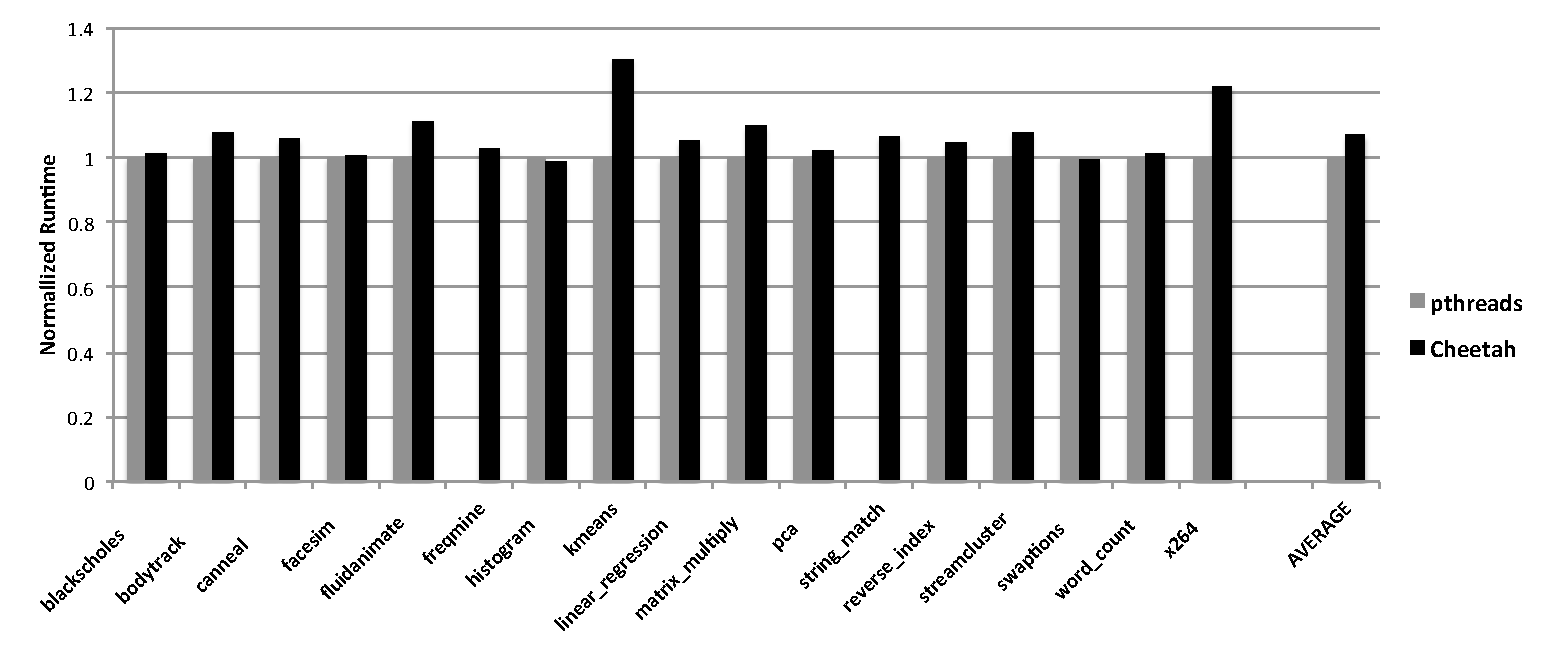
\includegraphics[width=2\columnwidth]{figure/Overhead.pdf}
\caption{Runtime overhead of \Cheetah{}. We normalize the runtime to that of \pthreads{}. On average, \cheetah{} only introduces around 7\% performance overhead on all evaluated applications, which makes it practical to be used in real deployment. \label{fig:overhead}}
\end{figure*}

We show the average runtime overhead of \cheetah{} in Figure~\ref{fig:overhead}. We run each application for five times and show the average results here. According to this figure, \cheetah{} only introduces around 7\% performance overhead, which makes it practical to be utilized in the real deployment. 

During the evaluation, we configure \cheetah{} with the sampling frequency at one out of 64K instructions. Thus, for every 64K instructions, the trap handler will be notified once so that \cheetah{} can collect the information of memory accesses on heap and global variables. Currently, \Cheetah{} skips memory accesses on kernel, libraries or others. 

The performance overhead of \cheetah{} mainly comes from the handling of each sampled memory access and each thread creation. For each sampled access, we will collect information such as the type of access (read or write), the number of cycles, and update  the history table of its corresponding cache line. \cheetah{} also intercepts every thread creation to setup the PMU unit, get the timestamp and update the phase information. For applications with a big number of threads, including \texttt{kmeans} (with 224 threads in 14 seconds) and \texttt{x264} (with 1024 threads in 40 seconds), setting PMU registers introduces non-negligible overhead since it invokes six \texttt{pfmon} APIs and six additional system calls. For other applications, \cheetah{} introduces less than 12\% performance overhead, with 4\% overhead on average if these two applications are excluded.  

%\todo{Check the creation of threads for kmeans and x264. Initializing IBS registers for every thread adds significant performance overhead. Kmeans 224 threads in 14 seconds. 1023 threads in 40 seconds.  }

%\todo{Should we check how the performance overhead will be changed at a different sample frequency?}
 
\subsection{Effectiveness}
\label{sec:effectiveness}

%The state-of-the-art tool Predator reports five false sharing instances in Phoenix and Parsec benchmark suite, including \texttt{histogram}, \texttt{linear\_regression}, \texttt{reverse\_index}, \texttt{streamcluster}, and \texttt{word\_count}~\cite{Predator}. 
\cheetah{} successfully detects two known false sharing problems with significant performance impact, including\texttt{linear\_regression} in Phoenix and \texttt{streamcluster} in PARSEC. 

%In the remaining of this section, we discuss how reported information can help us to confirm and fix these false sharing problems. 

%Finally, we study the false sharing that \cheetah{} does not detect in these benchmarks and verify that they have negligible impact to the overall program execution. 

\subsubsection{Case Study: linear\_regression}
Figure~\ref{fig:lr} shows the output of \cheetah{}. It points out that the {\tt tid\_args} object allocated at line 139, with the structure type {\tt lreg\_args}, incurs a severe false sharing problem. According to the assessment, fixing it can possibly improve the performance by $5.7\times$. By examining the source code, we can discover that the {\tt tid\_args} object is passed to different threads --- linear\_regression\_pthread. Then we can easily find out where false sharing has been exercised, which is shown as Figure~\ref{lr:code}. By checking word-based accesses that are reported by \cheetah{} but not shown here, we can understand the reason of this false sharing problem: different threads are updating different parts of the object {\tt tid\_args} simultaneously, where each thread updates words with the size of the structure lreg\_args. This problem is similar to the example shown in Figure~\ref{fig:penalty}. 

To address the problem, we pad the structure {\tt lreg\_args} with extra bytes, by adding 64 bytes useless content, so that we can force different threads not to access the same cache line. The one-line code change leads to a 5.7$\times$ speedup of the performance, which matches the assessment of 5.76$\times$ improvement predicted by \cheetah{}.

\begin{figure}
\begin{minipage}{\columnwidth}

\centering

\fbox
{
%\scriptsize
\begin{minipage}{3in}
Detecting false sharing at the object: start 0x400004b8 end 0x400044b8 (with size 4000). \\
Accesses 1263 invalidations 27f writes 501 total latency 102988 cycles.\\
\\
Latency information: \\
totalThreads 16 \\
totalThreadsAccesses 12e1 \\
totalThreadsCycles 106389 \\
%longestRuntime 7652 \\
%threadReduceRate 0.164697 \\
totalPossibleImprovementRate 576.172748\% \\
(realRuntime 7738 predictedRuntime 1343).\\
\\
It is a heap object with the following callsite:\\
linear\_regression-pthread.c: 139
\end{minipage}
}
\vspace{1em}
\caption{\cheetah{} reports a false sharing problem in \texttt{linear\_regression}.}
\label{fig:lr}
\end{minipage}
\end{figure}


\begin{figure}
%\scriptsize
\begin{verbatim}
typedef struct
{
  ......  
  long long SX;
  long long SY;
  long long SXX;
  ......
} lreg_args;	

for (i = 0; i < args->num_elems; i++)
{
  //Compute SX, SY, SYY, SXX, SXY
  args->SX  += args->points[i].x;
  args->SXX += args->points[i].x
              *args->points[i].x;
  args->SY  += args->points[i].y;
  ......
}
\end{verbatim}
\caption{The data structure and source code related to a serious false sharing instance in \texttt{linear\_regression}.}
\label{lr:code}
\end{figure}

\subsubsection{Case Study: streamcluster}

%Figure~\ref{fig:sc} shows the output of StreamCluster. 
We do not show the report results of streamcluster because of space limit. For streamcluster, every thread will update the \texttt{work\_mem} object concurrently, allocated at line 985 of the \texttt{streamcluster.cpp} file. The authors have already added some padding to avoid false sharing. However, they assume the size of cache line (as a macro) to be 32 bytes, which is smaller than the size of actual cache line used in our experimental machine. Thus, streamcluster will still have a significant false sharing problem. The performance impact of fixing false sharing problems inside is further discussed in Section~\ref{sec:precision}. 


\subsubsection{Comparing with State-of-the-art}

\begin{figure}[htbp]
\centering
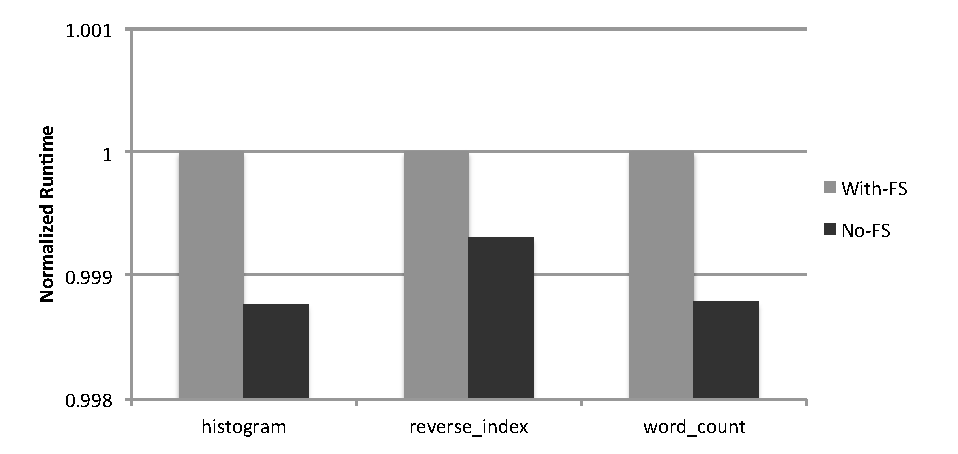
\includegraphics[width=1\columnwidth]{figure/trivial.pdf}
\caption{False sharing problems missed by \cheetah{} have negligible (<0.2\%) performance impact. \label{fig:fseffectiveness}}
\end{figure}

%\cheetah{} may miss some false sharing instances because of its sampling feature. 
Predator is the state-of-the-art in false sharing detection, which detects the most number of instances but with around $6\times$ performance overhead~\cite{Predator}. Comparing with Predator, \cheetah{} misses false sharing problems in \texttt{histogram}, \texttt{reverse\_index} and \texttt{word\_count}~\cite{Predator}. 

As discussed before, \cheetah{} only detects actual false sharing problems that may have significant performance impact on the final performance. If the number of accesses on a falsely-shared object is not large enough, \cheetah{} may not be able to detect it because of its sampling feature.  Also, the occurrences of false sharing can be affected by the starting address of objects or the size of the cache line or be affected by the cache hierarchy, as observed by Predator~\cite{Predator}. Thus, we further check the seriousness of these problems based on Predator's detection results. 

We run these applications on our experimental hardware, with and without false sharing problems. Figure~\ref{fig:fseffectiveness} shows the performance impact. Actually, these benchmarks do not show a significant speedup after fixing, with less than 0.2\% performance improvement. This behavior actually exemplifies the advantage of \Cheetah{}: since \cheetah{} only reports false sharing problems with significant performance impact, it can potentially save programmers manual effort unnecessarily spending on applications with trivial performance improvement. 

\subsection{Assessment Precision}
\label{sec:precision}

\cheetah{} is the first tool that can assess the performance impact of false sharing problems. Based on this information, programmers may save huge amount of manual effort spending unnecessarily on applications with trivial false sharing problems. 

We evaluate the precision of assessment on two applications that are detected to have false sharing problems, \texttt{linear\_regression} and \texttt{streamcluster}. We list the precision results in Table~\ref{tbl: precision}. In this table, \texttt{linear\_regression} is abbreviated as ``\texttt{linear\_reg}''.  We evaluate these applications when the number of threads is equal to 16, 8, 4, and 2 correspondingly. We list the predicted performance impact in the ``Predict'' column and the actual improvement in the ``Real'' column of the table. The last column (``Diff'') of this table lists the difference between the predicted improvement and the real improvement. If the number is larger than 0, the predicted performance improvement is less than the real improvement. Otherwise, it is the opposite. 
%The difference is calculated by dividing the difference by the real improvement.  

Table~\ref{tbl: precision} shows that \cheetah{} can perfectly assess the performance impact of false sharing in every case, with less than 10\% difference for every evaluated execution. %Relying on the assessment, programmers do not have to spend time on trivial false sharing problems any more. 
%\emph{According to this novel assessment of \cheetah{}, programmers may save huge amount of manual effort spending unnecessarily on applications with trivial false sharing problems}. 

\begin{table}
  \small
  \centering
  \begin{tabular}{ c | c | c | c | c}
  \hline
  \textbf{Application} & \specialcell{Threads \\ (\#)} & \textbf{Predict} & \textbf{Real} & \specialcell{Diff \\ (\%)}\\ \hline
\texttt{linear\_reg} & 16 & 6.44X    & 6.7X & {-3.8}\\
\texttt{linear\_reg}& 8  & 5.56X    & 5.4X & {+3.0}\\
\texttt{linear\_reg} & 4  & 3.86X  & 4.1X  & {-5.8}\\
 \texttt{linear\_reg}& 2  & 2.18X  & 2X    & {+9}\\ \hline
 \texttt{streamcluster} & 16 & 1.016X    & 1.015X &  {0}\\
 \texttt{streamcluster} & 8 & 1.017X    & 1.018X & {0}\\
 \texttt{streamcluster} & 4 & 1.024X    & 1.022X & {0}\\
 \texttt{streamcluster} & 2 & 1.033X    & 1.035X & {0}
 %\hline
\end{tabular}
  \caption{
    Precision of assessment. \Cheetah{} implements the first method to accurately predict the performance improvement of fixing an observed false sharing instance. \label{tbl: precision}}
\end{table}



%\section{Discussion}
\section{Discussion}

\label{sec:discuss}

This section addresses some possible concerns related to \Cheetah{}. 

\paragraph{Hardware Dependence.} \cheetah{} is an approach that relies on the hardware PMU unit to sample memory accesses. To use \cheetah{}, users should setup the PMU-based sampling beforehand. After that, they can connect to the library with the detection, prediction, and reporting component by calling only one API. Users should add the initialization of PMU at startup or in the begin of every thread, with adding less than 10 lines of code. Currently, we have implemented the hardware support for the AMD Opteron machine and plan to extend the support to Intel PEBS-related machines. 

\paragraph{Performance Overhead.} On average, \Cheetah{} only introduces 7\% performance overhead for all evaluated applications. However, \cheetah{} does introduce more than 20\% overhead for two applications with a large number of threads because \cheetah{} should setup hardware registers for every thread. Although creating a large number of threads in an application is not normal, we expect to only setup once with better hardware support. We also expect that the overhead can be further reduced by only sampling memory accesses, but not non-related instructions such as arithmetic instructions and logic instructions. Hopefully, the hardware can overcome these two limitations in the future.

\paragraph{Effectiveness.} \Cheetah{} can effectively detect false sharing problems that occur in the current execution and have high impact on the performance. For the effective detection, \Cheetah{} requires programs to run sufficient time, maybe more than few seconds. 


\section{Related Work}

\label{sec:relatedwork}
\cheetah{} is the first paper that attempts to predict the potential performance improvement after fixing an existing false sharing problem, by utilizing the access cycles provided by the PMU hardware.  Some prior work tends to breakdown the overhead of parallelization or stalls of cycles into different parts of programs or different hardware unit~\cite{Crovella:1994:PPP:602770.602870, Azimi:2005:OPA:1088149.1088163}, but we did not find any work that is close to our target. 

In this section, we will review existing tools for detecting false sharing issues, and other lightweight techniques for identifying memory bottlenecks of programs.

\subsection{False Sharing Detection}

Existing tools in false sharing detection can be classified into few different types, based on the way of collecting memory accesses or cache related events. 

\paragraph{Simulation Based Approaches.} Simulation based approaches try to simulate the behavior of program executions and predict possible problems inside~\cite{falseshare:simulator}. It relies on the input of programmers about specific cache hierarchy and hardware configurations. However, this types of tools will share the same shortcomings as other simulation based approaches: it can cause more than $100\times$ performance degradation; sometimes the results can be far from the real truth; it is hard to scale up to real applications with millions lines of code. 

% Simulation Based approaches. 

% Instrumentation Based Approaches
\paragraph{Instrumentation Based Approaches.} Many tools fall into this category. They can be further classified into dynamic instrumentation based approaches~\cite{falseshare:binaryinstrumentation1, falseshare:binaryinstrumentation2, qinzhao}, and static or compiler-based instrumentation based approaches~\cite{Predator}. Dynamic instrumentation based approaches do not need the availability of source code, but may fail to report the exact lines of problems if debugging related information does not exist in the binary file. Their performance can vary dramatically, from around $5\times$ slower ~\cite{qinzhao} to more than $100\times$ slower~\cite{falseshare:binaryinstrumentation1, falseshare:binaryinstrumentation2}. Compiler-based instrumentation can have better performance,  but needs the availability of source code and can not work on legacy programs without the source code~\cite{Predator}. However, all of existing tools introduces more than $5\times$ performance overhead and can not be used in real deployment. 

% Hardware performance based approaches
\paragraph{OS Related Approaches.} Sheriff proposes to turn threads into processes, relies on page protection and isolation to capture memory writes, and reports write-write false sharing problems with reasonable overhead (around 20\%)~\cite{Sheriff}. Plastic provides a VMM-based prototype system that combines the Performance Counter Monitoring (PMU) and page granularity analysis (based on page protection) to narrow down the problems of false sharing problems~\cite{OSdetection}. Both Sheriff and Plastic can automatically tolerate serious false sharing problems as well. However, both of them have their own shortcomings: Sheriff can only work on programs using \texttt{pthreads} libraries, and without ad-hoc synchronizations and sharing-the-stack accesses; Plastic requires that programs should run on the virtual machine environment, which is not the truth for most applications.   

\paragraph{PMU-based approaches.} In order to improve the performance and remove the necessity of source code, more and more tools turns to the hardware support to detect false sharing problems. Jayasena et. al. proposes to collect different types of events like memory accesses, data caches, TLBs, interactions among cores, and resources stalls, and uses the machine learning approach to derive potential memory patterns that can cause false sharing~\cite{mldetect}. However, they misses a lot of false sharing problems. DARWIN collects cache coherence events at the first round, then identifies possible memory accesses on data structures that are involved in frequent cache invalidations for the second round~\cite{openmp}. DARWIN also requires manual effort or expertise to verify whether false sharing occurs or not. Intel's PTU also relies on memory sampling mechanism but can not differentiate false sharing and true sharing since it discards the temporal information of memory accesses and can not present the detailed memory accesses on a cache line~\cite{detect:ptu}. DProf helps programmers identify cache misses based on AMD's instruction-based sampling hardware~\cite{DProf}. DProf requires manual annotation to locate data types and object fields, and cannot detect false sharing when multiple objects reside on the same cache line. \\

\cheetah{} falls into the category of PMU-based approaches. But it avoids shortcomings of existing PMU-based tools: it does not rely manual annotation, or experts' expertise, or multiple executions to locate the problem; it won't have false positives. It overcomes the limitations of OS-related approaches and can be used for applications running on either VM or non-VM environment. Comparing to approaches of using simulation and instrumentation, it has very low performance overhead and make it practical to be used in the real deployment.   

\todo{mention it can work on the mysql.
 It is also the first work that can predict the performance impact of false sharing problems. }

\subsection{Other PMU Related Analysis}
%There are many tools to analyze memory related bottlenecks, not necessarily relate to false sharing problems. 
%By monitoring every memory access, prior tools can analyze memory related bottlenecks, such as SLO~\cite{SLO1}, Valgrind~\cite{Nethercote:2007:VFH:1250734.1250746}, and MemSpy~\cite{Martonosi92}, but they may incur hundreds of times slowdowns. Selectively monitoring memory accesses can still cause 3-5$\times$ overhead, like MACPO~\cite{macpo}. 

PMU related techniques are widely used to identify other performance problems, such as memory system behavior and data locality. Itzkowitz et. al. introduced the memory profiling to Sun ONE Studio, which can collect and analyze memory accesses in sequential programs and report measurement data related to annotated code segment~\cite{DBLP:conf/sc/ItzkowitzWAK03}. Buck and Hollingsworth developed Cache Scope to perform data-centric analysis by using Itanium2 event address registers (EAR)~\cite{DBLP:conf/sc/BuckH04}. Cache Scope associates latency with data objects and functions that accessed them. HPCToolkit~\cite{ibs-sc} uses Intel PEBS and AMD IBS to associate performance metrics with both static and heap allocated data objects. It identifies problematic data objects with poor cache locality and long access latency. With similar techniques, ArrayTool~\cite{ibs-pact} further analyzes the samples collected by HPCToolkit to provide optimization guidance for array regrouping.

These tools have low overhead, typically less than 10\%, because of using PMU registers. Existing tools may point out a data object suffering with high access latency, but they can not tell whether the high latency comes from false sharing or not. In contrast, \cheetah{} can correctly identify false sharing problems and associate with problematic data objects.

% Comments: we will add this in the final version. But there is no need to add this since it haven't been published yet. 
% ScaAnalyzer~\cite{ibs-sc2} studies memory scalability in multithreaded programs. As false sharing is a kind of memory scalability bottleneck, ScaAnalyzer can pinpoint it and assess its impact with the increasing number of cores. 



%\subsection{Performance Prediction}

%Crovella et. al. provides a method to breakdown the aggregate seconds of parallel overhead into different categories, like serial fraction, synchronization, communication and contention\cite{Crovella:1994:PPP:602770.602870}. Azimi et. al. developed a Statistical Stall Break-down(SSB) model that can quantify the impact of each hardware component, e.g. caches, branch predictor, or other units, on the overall stall~\cite{Azimi:2005:OPA:1088149.1088163}. %\cite{Crovella:1994:PPP:602770.602870} the distinction between productive computation and parallel overhead is useful for both performance diagnosis  and performance prediction. It provides a method to further breakdown the aggregate seconds of parallel overhead into categories like serial fraction, synchronization, communication and contention.  
% Very closed ones:
% http://dl.acm.org/citation.cfm?id=602870 (we should find al related work on this)
% A Framework for Performance Modeling and Prediction
% http://dl.acm.org/citation.cfm?id=1088163
% http://onlinelibrary.wiley.com/doi/10.1002/cpe.1551/full
% http://link.springer.com/chapter/10.1007/978-3-642-14122-5_23
% 
% What is the idea of performance prediction? 
% How to predict? 
%There is no much work in performance prediction. Balsamo et. al.~\cite{Balsamo:2004:MPP:987527.987640} presents an overview on performance prediction on software systems. Fahringer et. al. proposes to predict the performance on distributed memory multiprocessor systems, by relying on compiler analysis. hihi ~\cite{Balsamo:2004:MPP:987527.987640} presents some recent researches that tries to use performance models to quantitatively predict the behavior of software system in the early-phase of development. 

%hihi ~\cite{impactofsharing}
%hihi~\cite{Joao:2012:BIS:2150976.2151001} 

%We are going to utilize the prediction technique that we are utilized to predict the more complicated thread model, not just fork-join models. 



% eliminate global lock
% possibly adopting a page-ownership protocol as used by ...

\section{Conclusions and Future Work}
\label{sec:conclusion}

In this paper, we present \cheetah{}, a lightweight profiler that precisely identifies false sharing in multithreaded programs. \cheetah{} 


{
\bibliographystyle{abbrv}
\bibliography{ref,tongping,datacentric}
}

\end{document}
